% ============================================================
% Engineering Project Report Template
% Adaptado para relatório técnico de engenharia IEEE
% PC4 — H-DROP: Módulo logístico autônomo de entrega
% ============================================================

\documentclass[12pt,a4paper]{article}

% ---------- Language / Encoding ----------
\usepackage[brazilian]{babel}
\usepackage[T1]{fontenc}
\usepackage[utf8]{inputenc}

% ---------- Page / Typography ----------
\usepackage{geometry}
\geometry{left=25mm,right=25mm,top=25mm,bottom=25mm}
\usepackage{setspace}
\setstretch{1.08}
\usepackage[protrusion=true,expansion=false]{microtype}

% ---------- Math / Units ----------
\usepackage{amsmath,amssymb}
\usepackage{siunitx}

% ---------- Figures / Tables ----------
\usepackage{graphicx}
\usepackage{float}
\usepackage{booktabs}
\usepackage{tabularx}
\usepackage{longtable}
\usepackage[table]{xcolor}

% Pasta das imagens (subpasta "Imagens e LIB") + raiz, para compilacao local
\graphicspath{{Imagens e LIB/}{./}}

% Fallback p/ imagem ausente: desenha caixa rotulada em vez de quebrar a compilacao.
% Ao adicionar a imagem real na subpasta, ela passa a aparecer automaticamente.
\let\origincludegraphics\includegraphics
\renewcommand{\includegraphics}[2][]{%
  \IfFileExists{Imagens e LIB/#2}{\origincludegraphics[#1]{#2}}{%
    \IfFileExists{#2}{\origincludegraphics[#1]{#2}}{%
      \fbox{\parbox[c][3cm][c]{0.6\textwidth}{\centering\ttfamily\footnotesize%
        [IMAGEM AUSENTE]\\\detokenize{#2}}}}}%
}

% ---------- Links / References ----------
\usepackage[hidelinks]{hyperref}
\usepackage{indentfirst}
\setlength{\parindent}{1cm}
\renewcommand{\labelitemii}{$\circ$}

% ---------- Code listings ----------
\usepackage{listings}
\lstset{
  basicstyle=\ttfamily\small,
  breaklines=true,
  frame=single,
}

% ---------- IEEE-style references ----------
\usepackage{csquotes}
\usepackage[backend=biber,style=ieee]{biblatex}
\addbibresource{Imagens e LIB/referencias.bib}

\usepackage{authblk}

% ============================================================
\title{\textbf{Automação e Robótica -- Relatório Técnico de Projeto [PC4]}\\
\vspace{0.5cm}
\large Título do Projeto: H-DROP - Módulo logístico autônomo de entrega}

\author{Diogo Freitas Machado, Elisa Nunes de Freitas, Gustavo Martins Gripaldi, Mayron Malaquias Oliveira, Pedro Borges Alves}

\affil{Curso de Engenharia de Computação -- IESB}

\date{2026}

% ============================================================
\begin{document}
\maketitle

% ============================================================
\section{Resumo executivo}

O projeto H-DROP consiste em um Veículo de Superfície Autônomo (ASV) do tipo catamarã, concebido para logística humanitária e comercial em regiões de difícil acesso terrestre. Este relatório (PC4) registra o estágio final do desenvolvimento, no qual todos os subsistemas — estrutura física, propulsão, alimentação, sensoriamento, geolocalização e comunicação — foram integrados em uma única plataforma funcional e submetidos a testes de validação. A estrutura em PVC, com a torre de comunicação e sensoriamento montada, foi testada em ambiente aquático, confirmando flutuabilidade e estabilidade sob a carga real da eletrônica embarcada. Os dois motores BLDC foram sincronizados e acionados pela bateria LiFePO4; o sistema de alimentação foi integrado de forma definitiva a todos os módulos de processamento (ESP32 e Arduino); e o subsistema de comunicação móvel 4G com geolocalização GNSS foi validado em campo.

No âmbito do \textit{firmware}, o sistema opera sobre FreeRTOS com uma Máquina de Estados Finita (FSM), distribuída entre a ESP32 (controle, navegação e telemetria 4G/GNSS) e o Arduino Nano (sensoriamento anticolisão, pesagem e sinalização). A telemetria via MQTT e a Estação de Controle de Missão em Angular foram consolidadas e exercitadas em conjunto com o hardware embarcado. Este documento analisa criticamente os resultados obtidos na integração final, o grau de atendimento dos requisitos estabelecidos, as limitações remanescentes — em especial a sintonização fina do controle autônomo de navegação — e as direções para a evolução futura da solução.

\vspace{0.5cm}

\noindent \textbf{Palavras-chave:} Veículo de Superfície Autônomo (ASV); Logística autônoma; Sistemas embarcados; Navegação autônoma; Internet das Coisas (IoT); Telemetria; Controle PID; Gerenciamento energético; Sensoriamento inteligente; Comunicação 4G.

% ============================================================
\section{Introdução}

O avanço da robótica móvel tem impulsionado a criação de soluções logísticas versáteis, capazes de operar com eficiência onde a infraestrutura terrestre tradicional é limitada ou inexistente. O projeto H-DROP surge como um Veículo de Superfície Autônomo (ASV) do tipo catamarã, projetado para atuar em duas frentes estratégicas: como plataforma de suporte em missões humanitárias e como sistema de \textit{delivery} de alta confiabilidade. Inspirado por modelos de logística de empresas como Amazon e iFood, o H-DROP visa automatizar a entrega de produtos em comunidades costeiras, canais urbanos e regiões de difícil acesso, oferecendo uma alternativa ágil ao transporte convencional.

A demanda por esse tipo de sistema cresce tanto pela necessidade de assistência em eventos climáticos extremos, que isolam populações ribeirinhas, quanto pela busca de eficiência logística em regiões sem infraestrutura terrestre. Enquanto drones aéreos sofrem restrições severas de capacidade de carga, o H-DROP utiliza uma estrutura robusta em PVC para transportar suprimentos com estabilidade, alternando entre o transporte de medicamentos em áreas de desastre e mercadorias de consumo diário com a mesma precisão operacional.

O desenvolvimento está alinhado aos conteúdos de controle discreto e sistemas embarcados da disciplina. A implementação exige uma plataforma microcontrolada para gerenciar a propulsão diferencial de motores \textit{brushless} e garantir que o ASV execute trajetórias autônomas de forma segura. Assim, o projeto consolida a integração de \textit{hardware} e \textit{software} para resolver um problema real de logística, transformando a via aquática em um canal de conectividade e suporte vital.

\textbf{Evolução desde os pontos de controle anteriores:} No PC1, o projeto estava em fase puramente conceitual, com modelagem matemática dos subsistemas, definição de requisitos e proposta arquitetural. No PC2, a transição para a prática revelou desafios reais: queima de um ESP32 por falha de soldagem, limitação do sensor ultrassônico único e dificuldades de manufatura do chassi em PVC. Esses desafios foram endereçados com correções técnicas documentadas. No PC3, o protótipo físico passou a existir e a flutuar, com seus principais subsistemas elétricos e de \textit{firmware} validados em bancada e em ensaios preliminares. No PC4 — estágio reportado neste documento — todos os subsistemas foram integrados em uma plataforma única: a torre de comunicação foi montada, o barramento de alimentação foi acoplado a todos os módulos de processamento (ESP32 e Arduino), os motores foram sincronizados, o enlace 4G/GNSS foi validado em campo e a embarcação completa foi ensaiada em ambiente aquático.

\textbf{Objetivo geral:} desenvolver e validar um Veículo de Superfície Autônomo de baixo custo, capaz de transportar carga útil entre dois pontos por navegação autônoma orientada por GNSS, com telemetria remota em tempo real via rede celular.

\noindent\textbf{Objetivos específicos:}
\begin{itemize}
\item construir uma plataforma flutuante estável (catamarã em PVC) com compartimento de carga estanque;
\item implementar propulsão diferencial por dois motores BLDC sincronizados via ESCs bidirecionais;
\item gerenciar a energia de um \textit{pack} LiFePO4 com BMS e estimativa de SoC por Contagem de Coulomb;
\item integrar geolocalização (GNSS) e orientação (magnetômetro) para navegação por \textit{waypoints};
\item prover comunicação móvel 4G com telemetria MQTT e Estação de Controle de Missão web;
\item dotar a embarcação de percepção anticolisão, pesagem de carga e sinalização visual de estado.
\end{itemize}

\textbf{Delimitação do escopo efetivamente implementado:} o trabalho entregou a plataforma física integrada, o subsistema energético, a propulsão sincronizada, a comunicação 4G/GNSS validada em campo e o \textit{firmware} de controle/telemetria, com ensaio da plataforma completa em água. A navegação autônoma ponto a ponto foi desenvolvida e exercitada em ambiente de simulação de alta fidelidade; a sintonização fina dos ganhos do controlador em malha fechada na água permanece como a principal frente de refinamento, discutida na Seção de Resultados.

% ============================================================
\section{Trabalhos Correlatos}

Para fundamentar as decisões de engenharia e a arquitetura do H-DROP, realizou-se um levantamento do estado da arte referente a Veículos de Superfície Autônomos (ASVs) e sistemas robóticos de logística. A revisão foi estruturada em eixos temáticos correspondentes aos principais subsistemas do projeto, avaliando para cada trabalho: o problema tratado, a solução proposta, a plataforma embarcada, a metodologia, os resultados e as limitações identificadas.

\subsection{Gerenciamento Energético e Controle de Navegação}

O estudo de Fernandes et al. (2025) \cite{fernandes2025smart} propõe Sistemas Inteligentes de Gerenciamento de Energia (SEMS) aplicados a ASVs em missões de vigilância de fronteiras. Os autores demonstram que a otimização do consumo durante o roteamento é essencial para estender a autonomia em ambientes sem infraestrutura de recarga. A plataforma utiliza baterias de lítio com monitoramento embarcado em tempo real. Como limitação, o sistema assume condições de navegação relativamente controladas. Esse trabalho fundamenta diretamente o algoritmo de Contagem de Coulomb via INA226 e a lógica de adaptação de velocidade baseada em SoC adotada no H-DROP.

A pesquisa de Sotelo-Torres et al. (2023) \cite{sotelo2023usv} aborda o desenvolvimento de um ASV de baixo custo para levantamentos batimétricos, utilizando propulsão diferencial via motores \textit{brushless} controlados por PWM e ESP32 como unidade central. Os resultados validam a capacidade do microcontrolador de traduzir comandos de navegação em manobras físicas responsivas em ambiente real. A limitação principal é a ausência de controle de energia embarcado. Esse trabalho corrobora diretamente as escolhas de \textit{hardware} de controle e propulsão do H-DROP.

\subsection{Estrutura Física e Propulsão}

Silva (2019) \cite{silva2019} utilizou Fluidodinâmica Computacional (CFD) para mapear a resistência ao avanço em embarcações do tipo catamarã. A autora confirma que a geometria multicasco é a mais eficiente para maximizar a flutuabilidade e estabilidade de rolagem em missões de carga. A metodologia CFD é robusta, porém exige recursos computacionais e tempo de modelagem inviáveis para o escopo do H-DROP. O trabalho sustenta a escolha da geometria de catamarã em PVC e o dimensionamento dos motores para superar o arrasto hidrodinâmico na velocidade de cruzeiro.

\subsection{Geolocalização e Roteamento}

Duran e Sonmez (2026) \cite{duran2026aquamib} apresentam o AquaMIB, um ASV voltado ao monitoramento de qualidade de água com georreferenciamento em tempo real. O sistema utiliza transceptores da fabricante SIMCom para transmitir coordenadas GNSS via rede celular 4G LTE. Os autores validam a precisão do georreferenciamento em ambientes aquáticos abertos. A principal limitação relatada é a perda de sinal em zonas de sombra. Esse resultado científico corrobora diretamente a adoção do módulo A7670SA no H-DROP.

\subsection{Comunicação Móvel e Plataforma de Acesso}

Al-Fuqaha et al. (2015) \cite{alfuqaha2015iot} realizam uma análise abrangente das tecnologias habilitadoras para IoT, enfatizando que o protocolo MQTT é fundamental para sistemas que operam sobre redes móveis, dado seu baixo \textit{overhead} frente ao HTTP. Embora o trabalho não trate especificamente de ASVs, a fundamentação teórica sobre o modelo \textit{publish/subscribe} sustenta a decisão arquitetural do H-DROP de utilizar MQTT sobre 4G LTE para telemetria.

\subsection{Sistema de Sensores e Percepção}

Bohn Júnior (2023) \cite{bohnjunior2023} aborda o desenvolvimento de embarcações não tripuladas de baixo custo para levantamentos hidrográficos em águas abrigadas, reforçando a importância da integração de sensores embarcados para navegação segura. O trabalho demonstra que sensores ultrassônicos são viáveis em ambiente aquático desde que adequadamente posicionados e filtrados por \textit{software}. Essa limitação — a dependência de posicionamento preciso — foi confirmada na prática pelo H-DROP durante o PC2, motivando a migração para um \textit{array} de três sensores JSN-SR04T em leque.

\subsection{Tabela Comparativa}

A Tabela \ref{tab:correlatos} sintetiza os trabalhos revisados e posiciona o H-DROP em relação a cada um.

\begin{table}[H]
\centering
\caption{Comparativo entre trabalhos correlatos e o H-DROP}
\label{tab:correlatos}
\renewcommand{\arraystretch}{1.3}
\small
\begin{tabularx}{\textwidth}{|p{2.2cm}|X|X|X|}
\hline
\rowcolor{gray!20}
\textbf{Trabalho} & \textbf{Foco principal} & \textbf{Limitação identificada} & \textbf{Diferencial do H-DROP} \\ \hline
Fernandes et al. (2025) & SEMS para missões de vigilância & Ambiente controlado, sem carga útil & Gestão energética acoplada à lógica de entrega logística \\ \hline
Sotelo-Torres et al. (2023) & Propulsão diferencial e controle & Sem gerenciamento de energia embarcado & Integração do subsistema energético com controle PID \\ \hline
Silva (2019) & Hidrodinâmica por CFD & Metodologia inacessível a baixo custo & Validação empírica com ensaios físicos em piscina \\ \hline
Duran \& Sonmez (2026) & Georreferenciamento em ASV & Perda de sinal em zonas cegas & Sistema com persistência de dados e \textit{buffer} local \\ \hline
Al-Fuqaha et al. (2015) & Protocolos IoT & Não trata de ASVs especificamente & Aplicação de MQTT em contexto náutico de baixo custo \\ \hline
Bohn Júnior (2023) & ASV de baixo custo & Sensor único com pontos cegos & \textit{Array} de sensores com filtragem por média móvel \\ \hline
\end{tabularx}
\end{table}

% ============================================================
\section{Fundamentação Teórica}

\subsection{Estrutura Física e Hidrodinâmica}

A topologia de catamarã foi selecionada por oferecer elevada estabilidade transversal sem a necessidade de lastros pesados. Dois cascos paralelos de PVC (diâmetro 100~mm, comprimento 1{,}0~m) são unidos por um chassi em tubos de 25~mm, conferindo rigidez torcional. A resistência hidrodinâmica ao avanço é dada por:
\begin{equation}
F_{drag} = \frac{1}{2} \cdot \rho \cdot v^2 \cdot S \cdot C_{T}
\end{equation}
onde $\rho$ é a densidade da água, $v$ a velocidade relativa, $S$ a área molhada e $C_{T}$ o coeficiente de resistência total. O volume deslocado pelos dois cascos é:
\begin{equation}
V_d = 2 \cdot \pi \cdot r^2 \cdot L \approx 0{,}01571 \text{ m}^3
\end{equation}
resultando em empuxo máximo de aproximadamente $154$~N ($\approx 15{,}7$~kg). Com a adição das proas em garrafas PET (contribuição de 0,73~kg) e flutuadores de EVA previstos ($+$5~kg), a reserva de flutuabilidade atinge 43{,}3\% sobre a massa operacional estimada de 15~kg, superando a margem de projeto de 40\% recomendada pela literatura.

A propulsão diferencial elimina a necessidade de leme físico. O momento de guinada (\textit{yaw}) é gerado pela diferença de empuxo entre os propulsores:
\begin{equation}
M_z = (F_{dir} - F_{esq}) \cdot \frac{d}{2}
\end{equation}
onde $d$ é a distância entre os eixos dos motores. As equações de avanço linear e guinada do corpo rígido descrevem o movimento:
\begin{equation}
m \cdot \dot{v} = (T_L + T_R) - F_{drag}
\end{equation}
\begin{equation}
J \cdot \dot{\omega} = \frac{d}{2}(T_R - T_L) - B\omega
\end{equation}

\subsection{Sistema de Alimentação Energética}

A tecnologia LiFePO4 foi selecionada após análise comparativa com baterias de chumbo-ácido e Li-Po. Suas vantagens determinantes são a curva de descarga praticamente plana (3{,}2~V por célula entre 20\% e 80\% de capacidade), segurança térmica intrínseca e vida útil superior a 2000 ciclos. O \textit{pack} 4S de 15~Ah fornece tensão nominal de 12{,}8~V e energia total de:
\begin{equation}
E_{total} = 12{,}8\text{ V} \times 15\text{ Ah} = 192\text{ Wh}
\end{equation}
Considerando profundidade de descarga (DoD) de 80\% para preservar a integridade química das células:
\begin{equation}
E_{util} = 192\text{ Wh} \times 0{,}8 \approx 153{,}6\text{ Wh}
\end{equation}
Com carga lógica de aproximadamente 6~W (ESP32, módulo 4G e sensores) e potência de propulsão em cruzeiro de 180~W, a autonomia estimada em missão contínua é:
\begin{equation}
T_{missao} = \frac{153{,}6\text{ Wh}}{180 + 6} \approx 0{,}83\text{ h (50 min)}
\end{equation}
Esse intervalo é superabundante para os ciclos de teste de campo previstos, que raramente excedem 15 a 20 minutos contínuos.

Como a curva de descarga da LiFePO4 é plana, a leitura de tensão é matematicamente ineficaz para estimar a autonomia. O método obrigatório é a \textbf{Contagem de Coulomb}:
\begin{equation}
SoC(t) = SoC(t_0) - \left(\frac{100}{C_{nom}}\right) \int_{t_0}^{t} I_{bat}(\tau)\, d\tau
\end{equation}
onde $C_{nom} = 15$~Ah e $I_{bat}$ é amostrado em tempo real pelo sensor INA226 via I2C.

A distribuição de potência segue uma cadeia Buck: a bateria alimenta os ESCs diretamente e, via conversor \textit{step-down}, fornece 5{,}0~V e 3{,}3~V para a lógica. Picos de corrente de até 2{,}8~A durante transmissões LTE são amortecidos por capacitores de tântalo de 1000~$\mu$F próximos ao módulo 4G.

\subsection{Controle Embarcado (ESP32 e FreeRTOS)}

O microcontrolador ESP32-WROOM-32 foi escolhido por seu processador dual-core Xtensa\textsuperscript{\textregistered} LX6 a até 240~MHz, com suporte nativo ao FreeRTOS. A arquitetura de software adota \textbf{Multiprocessamento Assimétrico (AMP)}: o Core~0 gerencia as tarefas de comunicação (UART, Wi-Fi) e o Core~1 executa exclusivamente a malha de controle PID. Esta separação garante determinismo temporal na malha de controle, imune a atrasos de rede.

O controlador PID digital é discretizado pelo método de Euler com período de amostragem $T_s = 50$~ms (20~Hz):
\begin{equation}
u[k] = K_p \cdot e[k] + I[k-1] + K_i \cdot T_s \cdot e[k] + \frac{K_d}{T_s}(e[k] - e[k-1])
\end{equation}
A proteção contra \textit{Integral Windup} é implementada por travamento condicional: a integração é suspensa quando o atuador está saturado. O sinal de saída é clampeado entre $u_{min}$ e $u_{max}$ e mapeado para o ciclo de trabalho do periférico MCPWM, que gera os pulsos a 50~Hz para os ESCs.

A cinemática inversa de navegação diferencial transforma o vetor de comando $(v, \omega)$ em velocidades individuais de cada motor:
\begin{equation}
V_R = v + \left(\omega \cdot \frac{L}{2}\right), \quad V_L = v - \left(\omega \cdot \frac{L}{2}\right)
\end{equation}
onde $L$ é a distância entre os centros dos cascos. O \textit{Soft-Start} impõe taxa de aceleração limitada:
\begin{equation}
\left|\frac{du(t)}{dt}\right| \le R_{max}
\end{equation}
garantindo corrente transitória máxima de 15~A por motor e proteção do \textit{pack} LiFePO4.

A FSM de energia define três modos de operação baseados estritamente no SoC: \textbf{Cruzeiro} (SoC $> 40\%$), no qual o ASV opera na velocidade planejada; \textbf{Eco} ($20\% <$ SoC $\le 40\%$), com redução de velocidade para maximizar o alcance; e \textbf{Parada de Segurança} (SoC $< 20\%$), que interrompe a propulsão e mantém apenas a telemetria ativa para retorno assistido. A transição entre modos é suavizada por histerese, evitando oscilação em regiões de fronteira.

Um \textbf{Watchdog de Comunicação} monitora o enlace entre o ESP32 e o módulo 4G. Se nenhum pacote UART válido for recebido por mais de 500~ms, o sistema entra em estado de parada segura (\textit{Failsafe}) e aciona sinalização de emergência conforme RIPEAM:
\begin{equation}
T_{atual} - T_{ultimo\_pacote} < T_{timeout} \quad (500\text{ ms})
\end{equation}

\subsection{Comunicação e Posicionamento (A7670SA)}

O módulo SIMCom A7670SA integra LTE Cat~1 e GNSS em um único fator de forma compacto, compatível com as bandas operadas na América Latina. A comunicação com o ESP32 ocorre via UART2 (GPIO 16/17) a 115200~bps, mediada por um conversor de nível bidirecional NPN que adapta os 3{,}3~V do ESP32 aos 1{,}8~V nominais do módulo. Um filtro RC ($R = 1$--$4{,}7\text{ k}\Omega$, $C = 1$~nF) na linha RX atenua \textit{spikes} de transição causados pelo atraso de corte dos transistores BJT.

A precisão do posicionamento é avaliada pela Diluição de Precisão Horizontal (HDOP). O sistema descarta leituras com HDOP $> 2{,}5$, pois esses valores indicam geometria de satélites desfavorável e erro posicional superior a 5~metros. O erro de posição horizontal é dado por:
\begin{equation}
E_h = HDOP \cdot \sigma_{UERE}
\end{equation}

Os dados de telemetria são empacotados em JSON e publicados via protocolo MQTT em um \textit{broker} dedicado (HiveMQ), que alimenta a Estação de Controle de Missão. A latência total ponta a ponta é modelada por:
\begin{equation}
L_{total} = L_{proc} + L_{network} + L_{broker} + L_{render}
\end{equation}
com requisito de latência média $\le 500$~ms.

\subsection{Sensoriamento e Percepção Ambiental}

A camada de sensoriamento integra quatro tipos de sensores:

\textbf{Ultrassom (JSN-SR04T):} Sensor à prova d'água com detecção de 0{,}2~m a 5{,}0~m. O lóbulo de irradiação de aproximadamente 20° revelou-se insuficiente com sensor único, levando à adoção de um \textit{array} de três sensores em leque para cobertura angular completa da proa. A distância medida é calculada por:
\begin{equation}
d_u = \frac{v_{som} \cdot \Delta t}{2}
\end{equation}
Um filtro de média móvel de 5 pontos é aplicado por \textit{firmware} para atenuar reflexões especulares na superfície da água.

\textbf{Magnetômetro (QMC5883L):} Fornece a proa magnética $\psi$ do ASV. Em baixas velocidades, o GNSS apresenta imprecisão direcional; a bússola digital supre essa lacuna com referência absoluta de orientação. O erro de proa é:
\begin{equation}
\epsilon_{\psi}(t) = \psi(t) - COG(t)
\end{equation}
onde $COG$ é o curso sobre o fundo fornecido pelo GNSS.

\textbf{Monitor de energia (INA226):} Amostra corrente e tensão via I2C a $\ge 10$~Hz, alimentando o algoritmo de Contagem de Coulomb e o protetor de subtensão (corte a 10{,}0~V, latência $\le 100$~ms).

\textbf{Célula de carga (HX711):} Opera em lógica binária (presença/ausência de carga), com limiar de detecção $V_{threshold}$ determinado empiricamente:
\begin{equation}
S_{load} = \begin{cases} 1, & \text{se } V_{load} > V_{threshold} \text{ (Ocupado)} \\ 0, & \text{se } V_{load} \le V_{threshold} \text{ (Vazio)} \end{cases}
\end{equation}

\subsection{Modelagem Completa do Sistema}

O vetor de medições do subsistema de sensores é:
\begin{equation}
\mathbf{y}(t) = \begin{bmatrix} d_u(t) \\ \psi(t) \\ V_{load}(t) \end{bmatrix}
\end{equation}

A navegação por \textit{waypoints} é baseada no erro espacial euclidiano:
\begin{equation}
E_p(t) = \sqrt{(x_{alvo} - x(t))^2 + (y_{alvo} - y(t))^2}
\end{equation}
O waypoint é considerado atingido quando $E_p(t) < \delta$, onde $\delta$ é o raio de tolerância GPS calibrado empiricamente. O tempo de transmissão serial para o módulo 4G é modelado por:
\begin{equation}
T_{tx} = \frac{S_{bytes} \cdot 10}{V_{baud}}
\end{equation}

% ============================================================
\section{Metodologia}

\subsection{Abordagem Geral de Desenvolvimento}

O H-DROP é desenvolvido de forma incremental e iterativa, com entregas parciais em Pontos de Controle (PC1 a PC4). A abordagem prioriza a validação independente de cada subsistema antes da integração total, reduzindo o risco de falhas sistêmicas em ambiente aquático.

\subsection{Etapas Executadas (PC3 ao PC4)}

O desenvolvimento foi organizado em três frentes simultâneas:

\begin{itemize}
\item \textbf{Simulação de Controle e Percepção (\textit{Software-in-the-Loop}):} Utilização da Estação de Controle e do \textit{broker} MQTT para injetar dados simulados de GNSS, magnetômetro e ultrassônico diretamente no ESP32. O objetivo foi validar a lógica PID, os filtros de média móvel e a máquina de estados de navegação antes do contato com a água.
\item \textbf{Integração Eletromecânica em Bancada:} União da bateria LiFePO4, BMS, INA226, ESCs e motores \textit{brushless} fora do ambiente aquático, com calibração do algoritmo de Contagem de Coulomb e implementação do \textit{throttling} por nível de carga.
\item \textbf{Montagem Estrutural do Catamarã:} Construção do chassi em PVC, instalação dos cascos, integração dos motores e ESCs, e realização dos primeiros ensaios hidrostáticos.
\item \textbf{Integração Final e Validação Aquática (PC4):} Montagem da torre de comunicação e sensoriamento, acoplamento definitivo do barramento de alimentação a todos os módulos de processamento (ESP32 e Arduino Nano), sincronização dos dois motores BLDC, validação do enlace 4G/GNSS em campo e ensaio da plataforma completa em ambiente aquático.
\end{itemize}

\subsection{Ferramentas Utilizadas}

As principais ferramentas adotadas foram: ESP-IDF com FreeRTOS para \textit{firmware} embarcado, Autodesk Fusion 360 para modelagem 3D e validação de proporções geométricas, Angular~19 com mapa Leaflet para a Estação de Controle de Missão, HiveMQ como \textit{broker} MQTT, e GitHub (\url{https://github.com/AlphaCompLabs/H-Drop}) como repositório do código-fonte.

\subsection{Organização da Equipe}

O projeto conta com cinco membros, cada um responsável por uma frente técnica, conforme a Tabela~\ref {tab:responsabilidades}: alimentação, propulsão, controle, estrutura física, sistema de software, sensores anticolisão e peso, elementos visuais, geolocalização e comunicação. As frentes são coordenadas em reuniões semanais com atualização de ata.

\begin{table}[H]
\centering
\begin{tabular}{|l|l|}
\hline
\textbf{Responsável} & \textbf{Frente Técnica} \\ \hline
Diogo Freitas    & Alimentação e Propulsão \\ \hline
Elisa Nunes      & Controle e Estrutura Física \\ \hline
Gustavo Martins  & Sistema de Software \\ \hline
Mayron Malaquias & Sensores Anticolisão e Peso; Elementos Visuais \\ \hline
Pedro Borges     & Geolocalização e Comunicação \\ \hline
\end{tabular}
\caption{Distribuição de responsabilidades técnicas por membro.}
\label{tab:responsabilidades}
\end{table}

\vspace{0.3em}
{\footnotesize \textit{Nota: algumas responsabilidades definidas no PC2 foram redesenhadas para melhor adequação à dinâmica de desenvolvimento da equipe.}}

\subsection{Estratégia de Testes}

Os testes seguem três estágios progressivos: (1) validação em bancada de cada subsistema isolado; (2) integração em \textit{Hardware-in-the-Loop} (HIL), simulando a carga hidrodinâmica eletronicamente; e (3) ensaios em ambiente aquático real, iniciados com testes estáticos de flutuabilidade e progredindo para missões autônomas completas.

% ============================================================
\section{Desenvolvimento}

\subsection{Arquitetura do Sistema}

A arquitetura do H-DROP é organizada em seis centrais funcionais interconectadas, conforme ilustrado na Figura \ref{fig:diagrama_controle_detalhado}.

\begin{figure}[H]
\centering
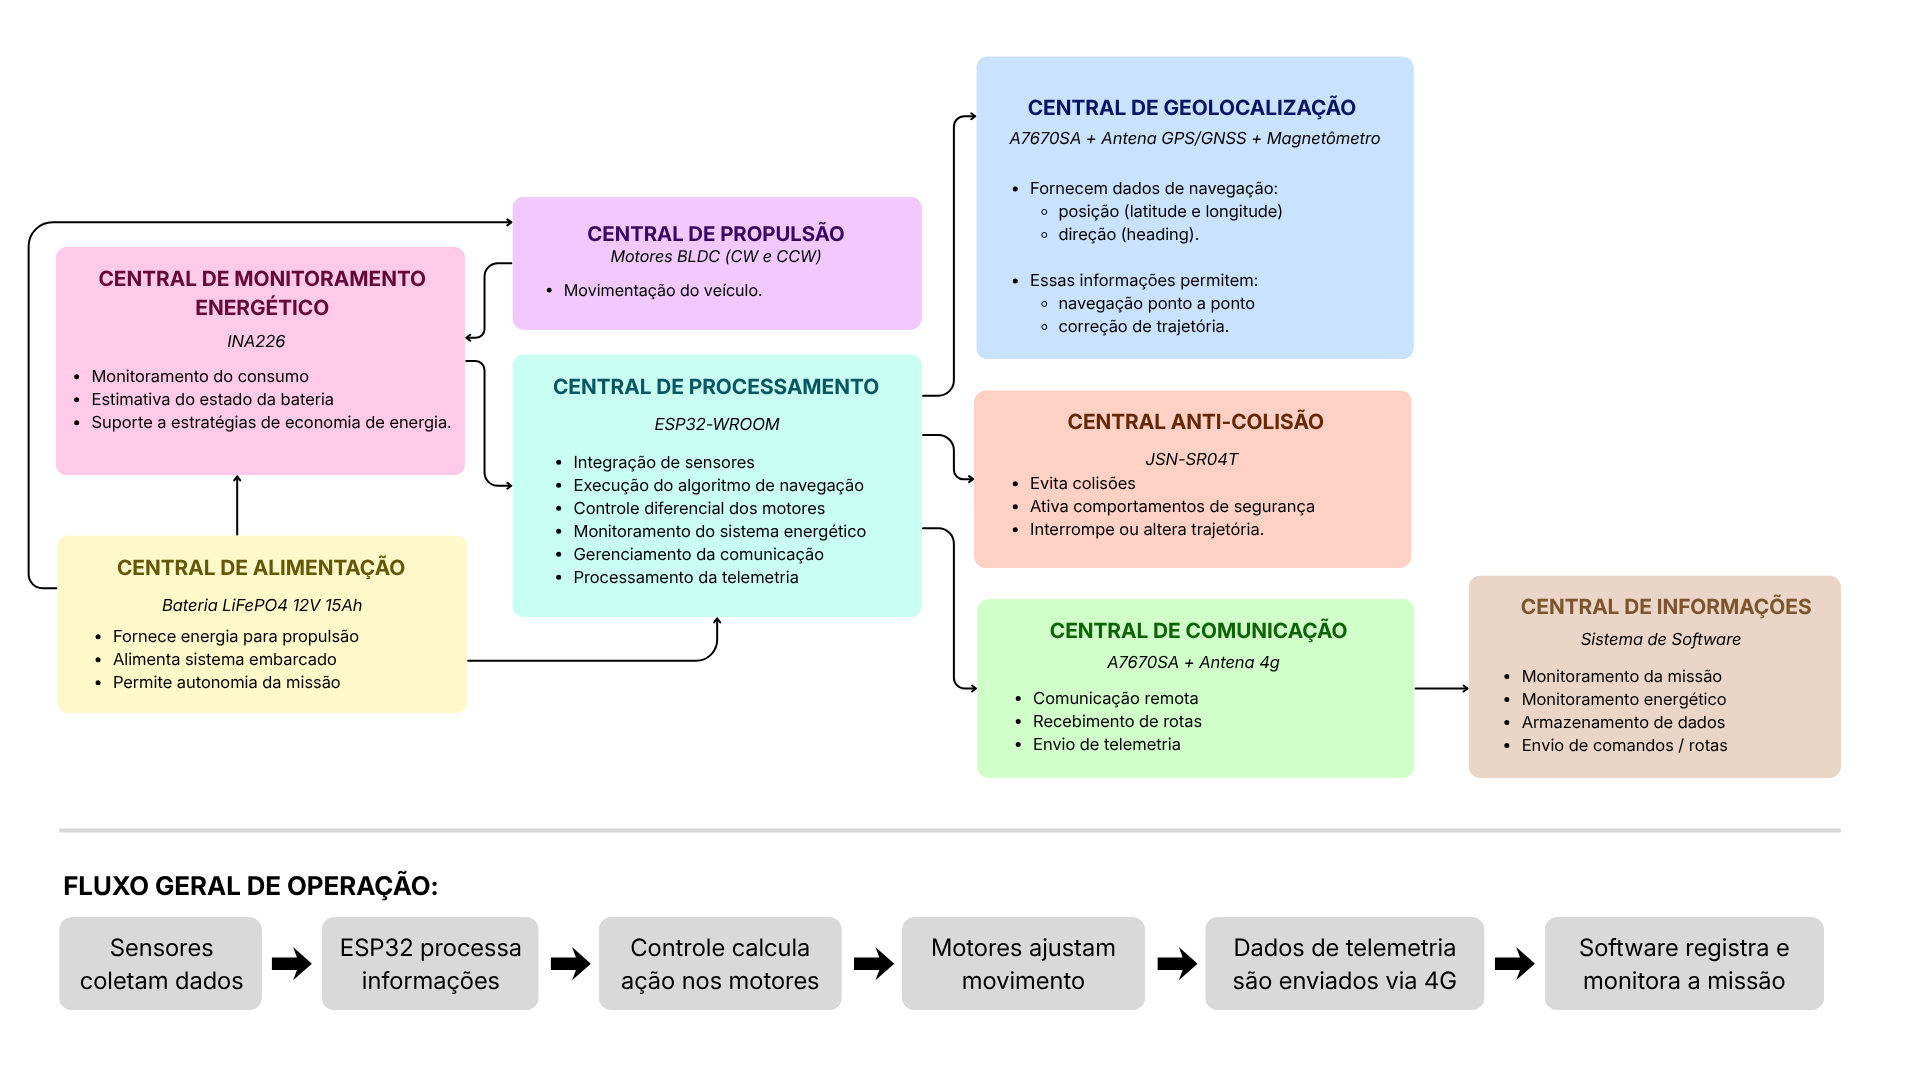
\includegraphics[width=0.85\textwidth]{Diagrama de Controle.png}
\caption{Diagrama de blocos da arquitetura de \textit{hardware} e fluxo de operação entre as centrais do sistema.}
\label{fig:diagrama_controle_detalhado}
\end{figure}

\begin{figure}[H]
\centering
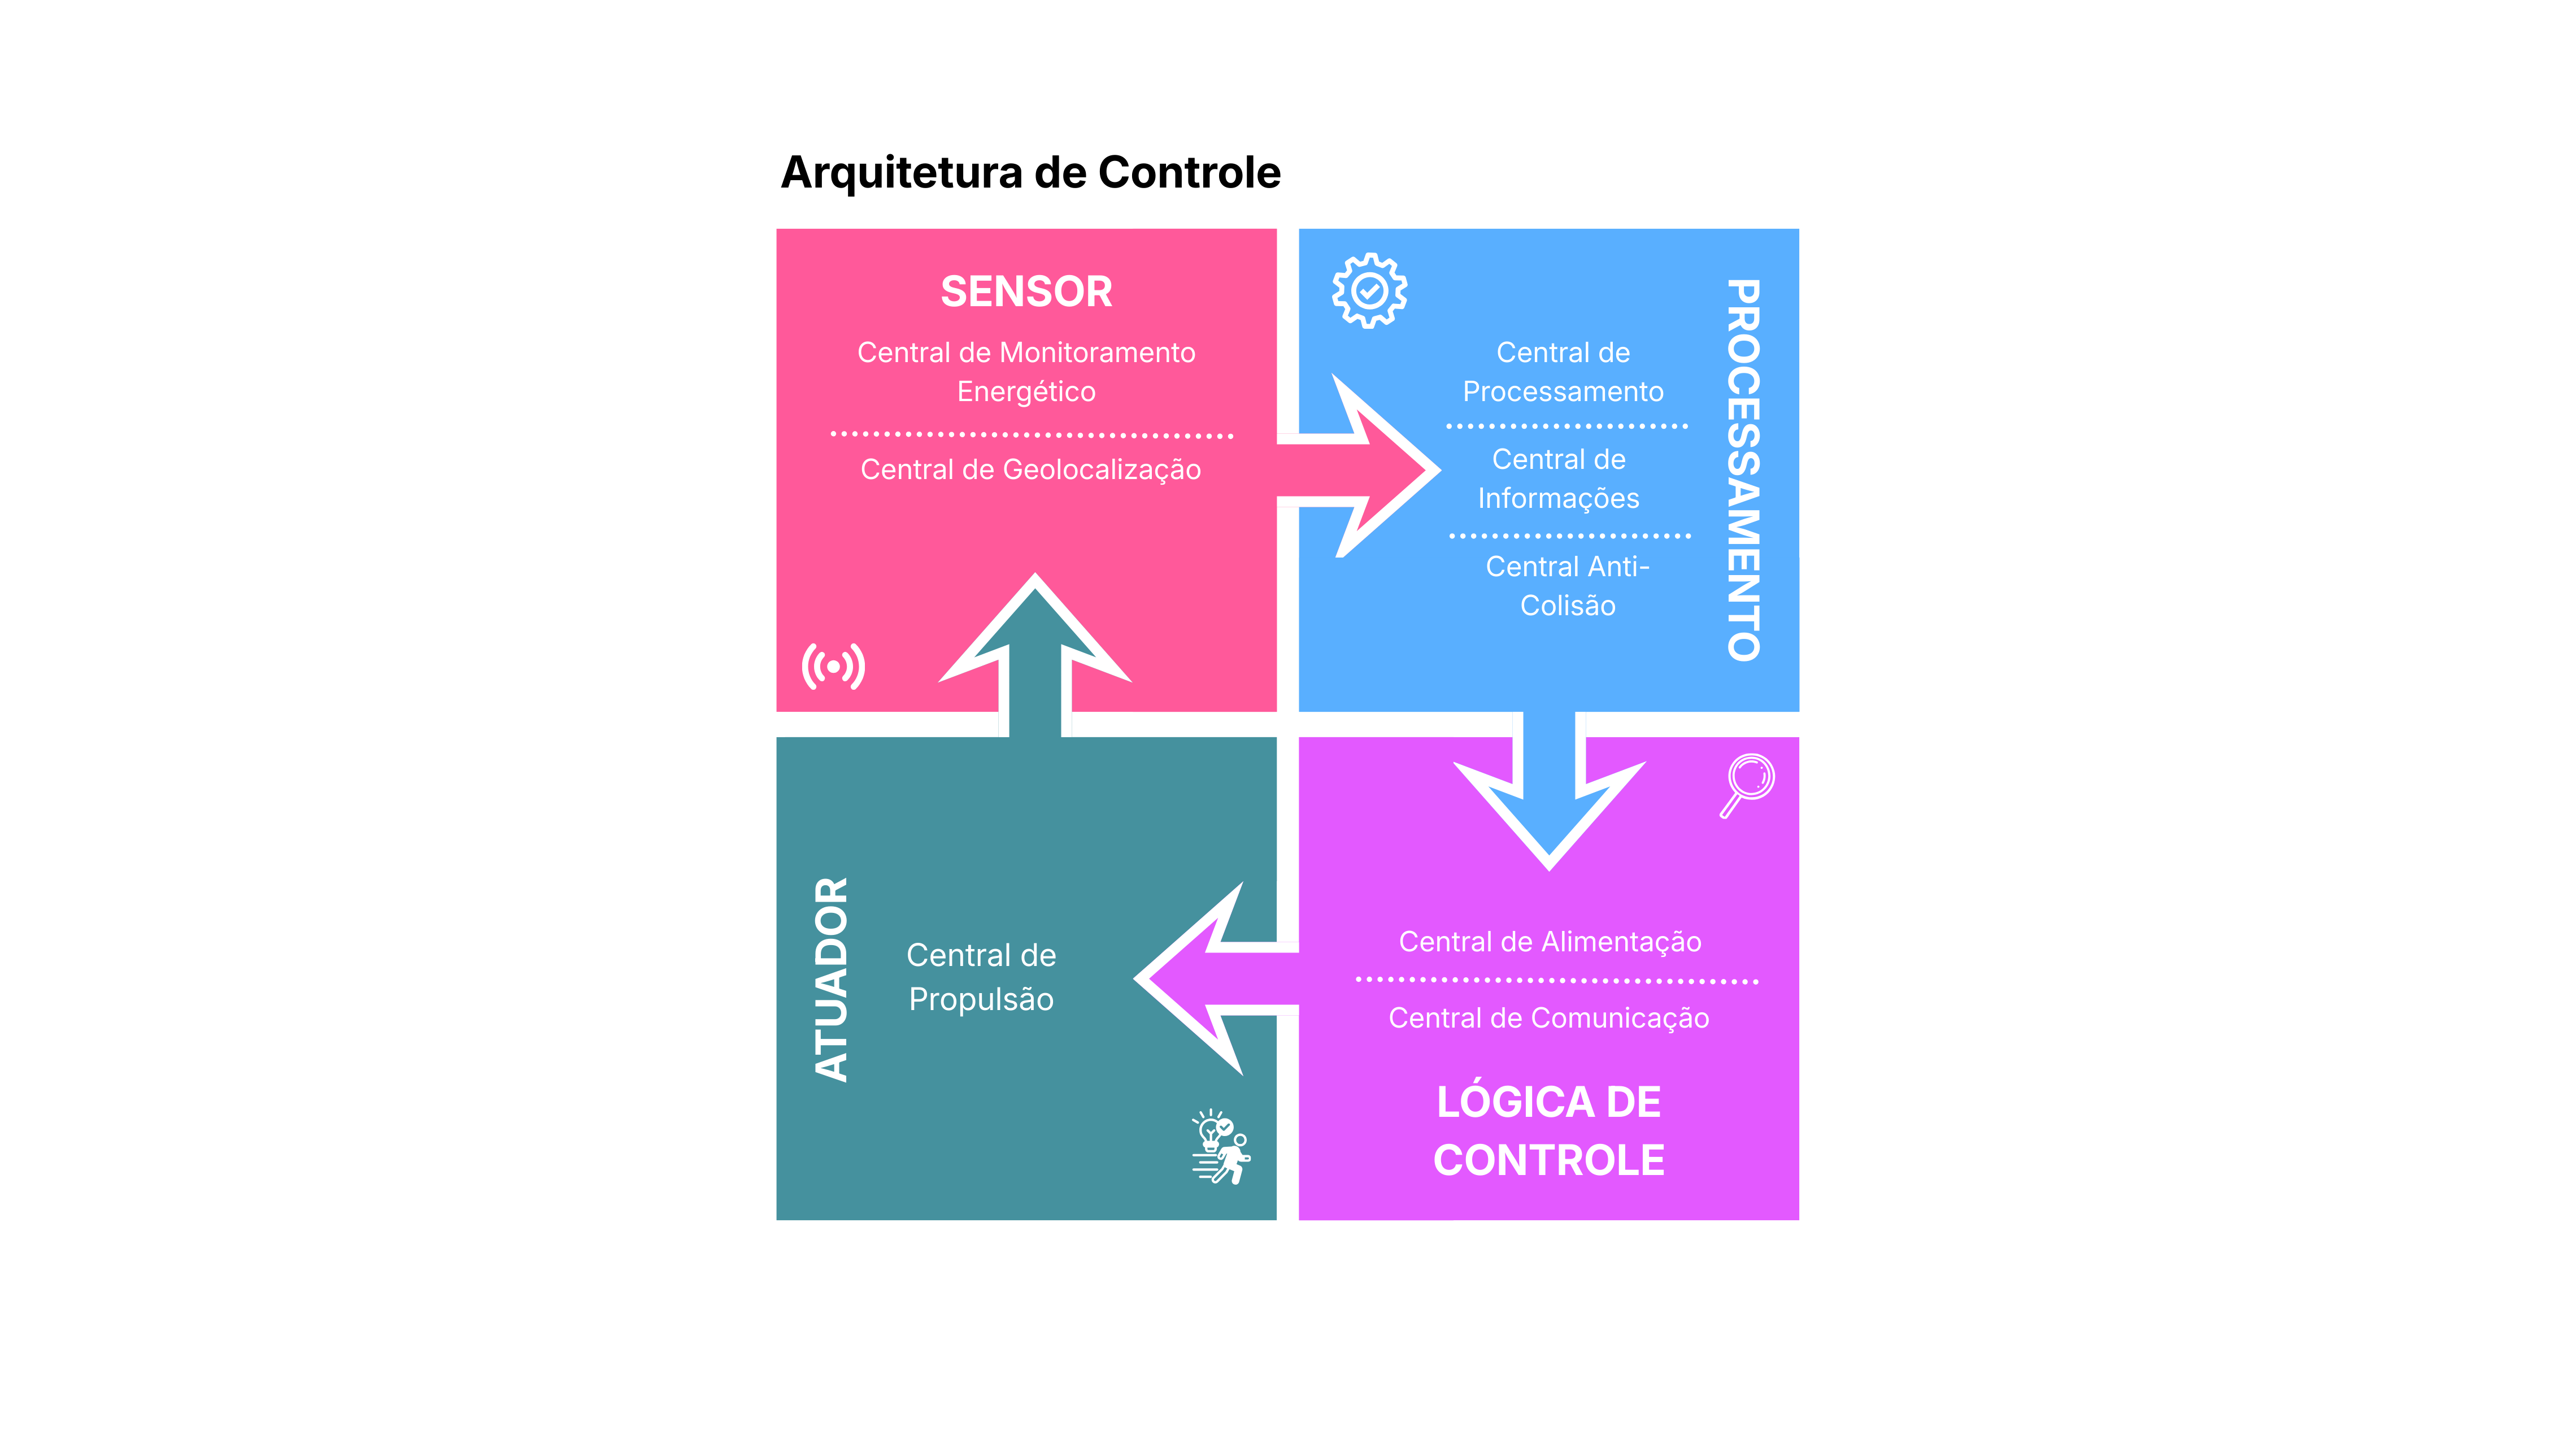
\includegraphics[width=0.75\textwidth]{Arquitetura de Controle.png}
\caption{Arquitetura de controle cíclica, abstraindo as centrais em eixos de Sensoriamento, Processamento, Lógica de Controle e Atuação.}
\label{fig:arquitetura_controle_ciclica}
\end{figure}

As seis centrais e suas responsabilidades são:

\begin{itemize}
\item \textbf{Central de Alimentação:} Bateria LiFePO4 4S (15~Ah) com BMS ativo, fornecendo energia para todos os subsistemas e permitindo autonomia de missão.
\item \textbf{Central de Propulsão:} Dois motores BLDC de 480~KV controlados por ESCs bidirecionais de 50~A, implementando propulsão diferencial e giro sobre o próprio eixo.
\item \textbf{Central de Processamento:} ESP32-WROOM-32 executando FreeRTOS, integrando sensores, calculando a malha PID, gerenciando a telemetria e supervisionando a energia.
\item \textbf{Central de Geolocalização:} Módulo A7670SA com antena GNSS ativa e magnetômetro QMC5883L, fornecendo posição, direção e fusão de dados para correção de proa.
\item \textbf{Central Anti-Colisão:} \textit{Array} de três sensores JSN-SR04T posicionados em leque na proa, cobrindo o plano frontal do ASV para evasão autônoma.
\item \textbf{Central de Comunicação:} Módulo A7670SA com antena 4G LTE, transmitindo telemetria via MQTT e recebendo waypoints e comandos da Estação de Controle remota.
\end{itemize}

\subsection{Hardware Implementado}

\subsubsection{Alimentação e Proteção Elétrica}
O sistema opera com uma topologia de múltiplos domínios de tensão. O barramento de potência é alimentado pela bateria LiFePO4 4S (10{,}0~V a 14{,}6~V), protegida ativamente pelo módulo BMS-4S de 30~A que realiza balanceamento celular e corte por subtensão. O barramento lógico é derivado via conversor Buck ajustado para 5{,}0~V e 3{,}3~V, garantindo eficiência $\ge 90\%$ e ondulação máxima de 50~mVpp.

\begin{figure}[H]
\centering
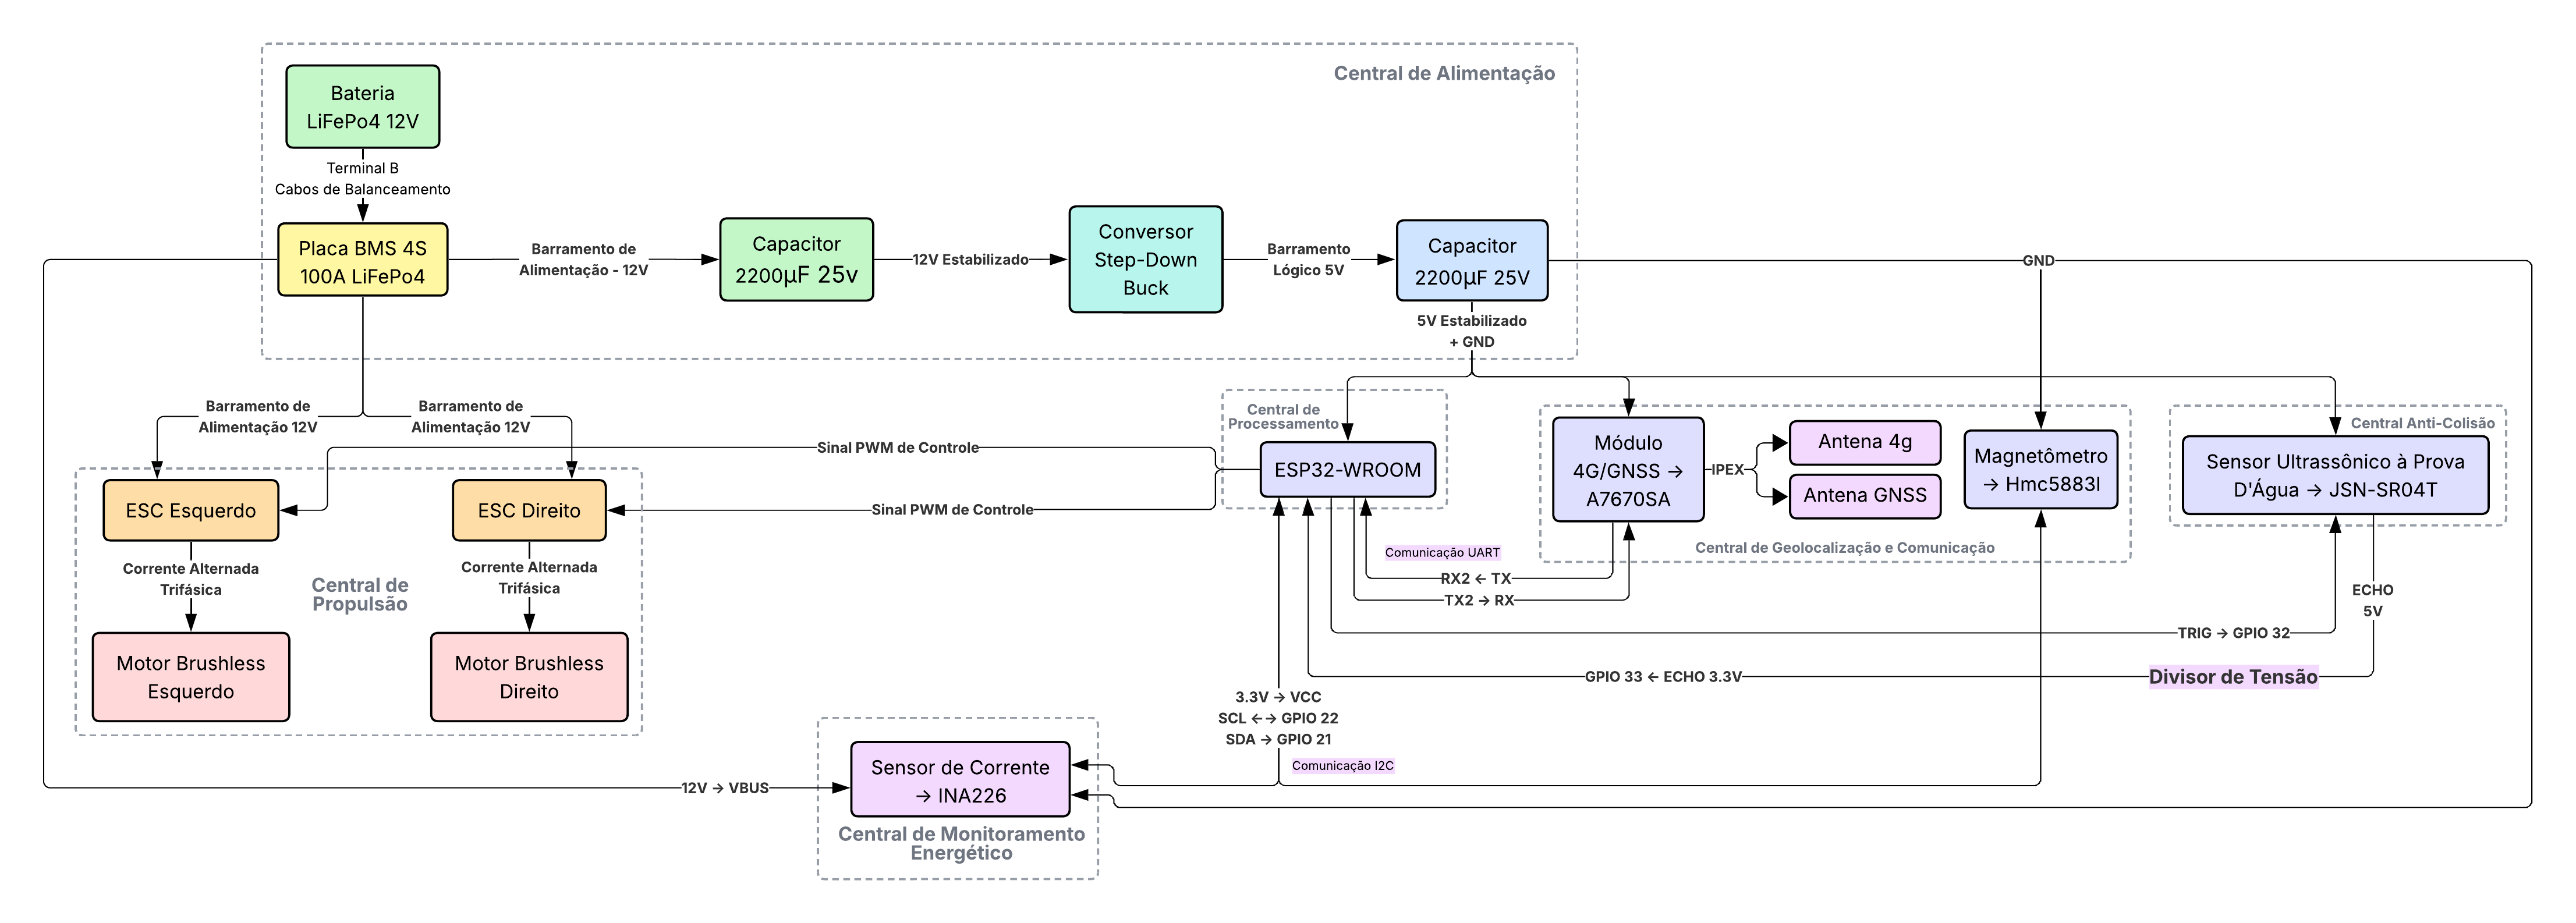
\includegraphics[width=0.85\textwidth]{esquematico_preliminar.png}
\caption{Esquemático do sistema de navegação e telemetria — versão atualizada PC3.}
\label{fig:esquematico_pc3}
\end{figure}

A compatibilidade entre o ESP32 (3{,}3~V) e o módulo A7670SA (1{,}8~V nominal) é assegurada por um conversor de nível NPN bidirecional. A linha de recepção (RX) recebe ainda um filtro RC passivo (resistor de 1~k$\Omega$ a 4{,}7~k$\Omega$ em série, capacitor de 1~nF ao GND) para atenuar os \textit{spikes} gerados pelo atraso de corte dos transistores BJT em 115200~bps. Os picos de corrente do 4G (até 2{,}8~A durante \textit{bursts} LTE) são amortecidos por capacitores de tântalo de 330~$\mu$F a 1000~$\mu$F próximos ao pino VBAT do módulo.

\subsubsection{Componentes Selecionados}

A Tabela \ref{tab:componentes_riscos} apresenta os componentes selecionados, com justificativas técnicas, riscos e custos.

\renewcommand{\arraystretch}{1.3}
\footnotesize
\begin{longtable}{|p{2.8cm}|p{5.0cm}|p{4.0cm}|c|r|}
\caption{Matriz de Componentes: Especificações, Riscos e Custos}
\label{tab:componentes_riscos} \\
\hline
\textbf{Componente} & \textbf{Justificativa e Especificação} & \textbf{Riscos e Observações} & \textbf{Qtd.} & \textbf{Custo (R\$)} \\ \hline
\endfirsthead
\multicolumn{5}{c}{{\tablename\ \thetable{} -- Continuação da página anterior}} \\
\hline
\textbf{Componente} & \textbf{Justificativa e Especificação} & \textbf{Riscos e Observações} & \textbf{Qtd.} & \textbf{Custo (R\$)} \\ \hline
\endhead
\hline \multicolumn{5}{|r|}{\textit{Continua na próxima página...}} \\ \hline
\endfoot
\hline
\endlastfoot

\multicolumn{5}{|c|}{\textbf{Estrutura Física}} \\ \hline
Tubos e Conexões de PVC (Kit) & Material leve, de fácil usinagem e alta flutuabilidade para os cascos. & Falha na colagem pode gerar infiltração e comprometer a eletrônica. & 01 & 126,48 \\ \hline

\multicolumn{5}{|c|}{\textbf{Controle, Alimentação e Propulsão}} \\ \hline
ESP32-WROOM-32D & Microcontrolador central; executa o PID e a lógica de navegação. & Limite de portas GPIO exige planejamento rígido de pinagem. & 01 & 38,70 \\ \hline
Bateria LiFePO4 12V 4S & Fonte de energia principal com química estável e alta durabilidade. & Risco de descarga profunda se a telemetria falhar. & 01 & 393,43 \\ \hline
BMS 4S 100A (Placa de Gestão) & Proteção contra sobrecarga e balanceamento das células da bateria. & Erro na fiação do chicote de balanceamento pode danificar o \textit{pack}. & 01 & 37,49 \\ \hline
Motores Brushless (Thrusters) & Propulsão submersível 12--24~V 20~A com empuxo diferencial. & Entrada de detritos na hélice pode causar travamento e queima. & 02 & 193,17 \\ \hline
ESCs 50A (Bidirecionais) & Controladores de velocidade com suporte a marcha-ré. & Necessidade de dissipação térmica dentro da caixa estanque. & 02 & 237,34 \\ \hline
Sensor INA226 + Resistor Shunt & Monitoramento de corrente, tensão e Contagem de Coulomb. & Aquecimento do \textit{shunt} em correntes altas; exige ventilação. & 01 & 37,00 \\ \hline
Step-Down Buck + Capacitores & Regulação de 5~V para a lógica e filtragem de ruído de potência. & Ruído residual pode causar instabilidade no GPS/4G. & 01 & 15,00 \\ \hline

\multicolumn{5}{|c|}{\textbf{Sensores de Colisões e Sinalização}} \\ \hline
JSN-SR04T (Ultrassônico) & À prova d'água, detecção de até 5~m. & Zona cega de 20~cm exige tratamento por \textit{software}. & 03 & 49,50 \\ \hline
MPU-6050 (Módulo Inercial) & Monitora a dinâmica e inclinação, prevenindo tombamento. & Sensível a vibração dos motores; requer filtro de Kalman. & 01 & 33,90 \\ \hline
Fita LED SMD3528 & \textit{Feedback} visual para identificar estados de navegação. & Risco de oxidação nos pontos de corte se não selados. & 01 & 39,90 \\ \hline
Célula de Carga (50~kg) + HX711 & Identifica presença de carga para validação logística. & Deformação permanente por torque excessivo na fixação. & 01 & 9,50 \\ \hline

\multicolumn{5}{|c|}{\textbf{Geolocalização e Comunicação}} \\ \hline
SIMCom A7670SA (Módulo 4G/GNSS) & Centraliza telemetria via rede celular e coordenadas globais. & Picos de corrente de até 2~A (mitigados por capacitor). & 01 & 120,80 \\ \hline
QMC5883L (Magnetômetro) & Bússola digital para controle de proa (\textit{heading}). & Interferência eletromagnética gerada por motores e ESCs. & 01 & 25,00 \\ \hline
Kit Antenas (4G + GNSS Ativa) & Garante ganho de sinal em áreas afastadas. & Atenuação dependendo da instalação no casco. & 01 & 43,52 \\ \hline
Level Shifter (Conversão Lógica) & Comunicação segura entre periféricos 5~V e ESP32 (3{,}3~V). & Erro de montagem pode causar queima do módulo 4G. & 01 & 15,00 \\ \hline

\hline
\multicolumn{4}{|r|}{\textbf{Total Estimado}} & \textbf{1.415,73} \\

\end{longtable}
\normalsize

\subsubsection{Organização Física dos Componentes}

O chassi é construído em tubos de PVC de 25~mm (estrutura), 50~mm (torre de sensores e extensões de popa) e 100~mm (cascos). A união dos cascos ao chassi é feita com fitas metálicas envoltas em câmara de ar de pneu, travadas com enforca-gatos de nylon, eliminando parafusos metálicos que gerariam interferência eletromagnética nas antenas. A torre de sensores possui 50~cm de altura acima do convés, posicionada na proa, garantindo linha de visada desobstruída para as antenas GNSS/4G e ângulo de incidência favorável para os sensores ultrassônicos.

O deck superior acomoda o compartimento de carga, estruturado para transportar os suprimentos com segurança e isolamento do ambiente aquático. Os ESCs são instalados sobre o chassi aberto para dissipação térmica passiva. A bateria é posicionada na base do deck central para minimizar o centro de gravidade e ampliar a estabilidade metacêntrica. O cabeamento estruturado percorre os cascos em fita isolante \textit{split loom}, afastado das linhas de dados para prevenir indução de ruído eletromagnético.


\subsection{Estratégia Experimental}

\subsubsection{Ensaios Hidrostáticos}

Os ensaios avaliam a flutuabilidade, o equilíbrio do centro de gravidade e a estanqueidade das conexões de PVC. O critério de aceitação é: empuxo total superior ao peso carregado e ângulo de inclinação estático $\le 15°$.

\subsubsection{Ensaios de Percepção}

Determinam experimentalmente a cobertura angular do \textit{array} de sensores ultrassônicos. Medições de distância são realizadas com anteparos fixos em solo e na água, verificando a faixa útil de 0{,}2~m a 5{,}0~m com erro máximo de 2\%.

\subsubsection{Ensaios de Malha Fechada}

Avaliam a capacidade do ASV de manter a velocidade de cruzeiro sob distúrbios externos (correntes, ventos) e de recalcular a rota após evasão de obstáculos, retomando a navegação orientada por \textit{waypoints} GNSS. A telemetria energética via MQTT é verificada em paralelo.

% ============================================================
\section{Requisitos Técnicos Consolidados}

A Tabela \ref{tab:requisitos_tecnicos} consolida todos os requisitos técnicos dos subsistemas, mantida e validada desde o PC1 com ajustes decorrentes das evoluções do PC2 e PC3.

\vspace{0.5cm}
\noindent\footnotesize\textbf{Legenda dos Subsistemas do Projeto:}\\
\textbf{GE}: Gerenciamento Energético \quad|\quad \textbf{CT}: Controle de Navegação \quad|\quad \textbf{EF}: Estrutura Física \quad|\quad \textbf{PR}: Propulsão \quad|\quad \textbf{GR}: Geolocalização e Roteamento \quad|\quad \textbf{CM}: Comunicação Móvel e Plataforma de Acesso \quad|\quad \textbf{SP}: Sensores e Percepção
\vspace{0.3cm}
\normalsize

\renewcommand{\arraystretch}{1.3}
{
\small
\begin{longtable}{| c | >{\raggedright\arraybackslash}p{0.14\textwidth} | >{\raggedright\arraybackslash}p{0.18\textwidth} | >{\raggedright\arraybackslash}p{0.22\textwidth} | >{\raggedright\arraybackslash}p{0.17\textwidth} | >{\raggedright\arraybackslash}p{0.14\textwidth} |}

\caption{Requisitos Técnicos dos Subsistemas do Projeto}
\label{tab:requisitos_tecnicos} \\

\hline
\textbf{Sub.} & \textbf{Requisito} & \textbf{Descrição} & \textbf{Justificativa Técnica} & \textbf{Métrica / Verificação} & \textbf{Valor Aceitável} \\ \hline
\endfirsthead
\multicolumn{6}{c}{{\bfseries Tabela \thetable{} -- Continuação da página anterior}} \\
\hline
\textbf{Sub.} & \textbf{Requisito} & \textbf{Descrição} & \textbf{Justificativa Técnica} & \textbf{Métrica / Verificação} & \textbf{Valor Aceitável} \\ \hline
\endhead
\hline \multicolumn{6}{|r|}{{\textit{Continua na próxima página...}}} \\ \hline
\endfoot
\hline
\endlastfoot

\textbf{GE} & Regulação de Tensão & Converter a tensão flutuante da bateria para níveis estáveis para microcontroladores e periféricos. & A tensão LiFePO4 4S varia de 10{,}0~V a 14{,}6~V. Conversores Buck previnem \textit{brownouts} que reiniciam o ESP32. & Medição de \textit{ripple} e queda de tensão sob carga máxima (propulsão + 4G ativos). & 5{,}0~V ($\pm 5\%$) e 3{,}3~V ($\pm 5\%$). Ondulação $\le 50$~mVpp. Eficiência $\ge 90\%$. \\ \hline

\textbf{GE} & Estimativa de SoC & Quantificar a energia consumida em tempo real via Contagem de Coulomb. & A curva de descarga LiFePO4 é plana; leitura de tensão é insuficiente. INA226 + integral no ESP32 são obrigatórios. & Comparação do SoC calculado com coulombímetro de bancada (descarga a 0{,}5C). & Erro de SoC $\le 5\%$. Aquisição I2C $\ge 10$~Hz. \\ \hline

\textbf{GE} & Proteção de Subtensão & Interromper propulsão ao atingir o limiar mínimo de tensão. & Células LiFePO4 sofrem degradação irreversível abaixo de 2{,}5~V/célula. & Teste com rampa decrescente de tensão; medir tempo até PWM zerar. & Corte em 10{,}0~V. Latência $\le 100$~ms. \\ \hline

\textbf{CT} & \textit{Soft-Start} & Limitar corrente de partida com aceleração gradual. & Picos de partida podem superar 30~A, causando \textit{voltage sag} e desarme do BMS. & Curva de corrente de partida com degrau de 0\% a 100\%. & Corrente transitória $\le 15$~A/motor. Rampa de 1 a 2~s. \\ \hline

\textbf{CT} & PID Malha Fechada & Estabilizar rotação e rastrear \textit{setpoint} de velocidade. & Dinâmica da água e queda de tensão são distúrbios contínuos. & Resposta ao degrau em água; tempo de acomodação e \textit{overshoot}. & \textit{Loop} PID $\ge 20$~Hz. \textit{Overshoot} $\le 10\%$. Erro de regime $\le 5\%$. \\ \hline

\textbf{CT} & Gestão de Energia por SoC & Adaptar a velocidade de cruzeiro conforme o Estado de Carga da bateria, preservando a autonomia da missão. & SoC calculado via Contagem de Coulomb define o modo de operação da FSM (Cruzeiro, Eco ou Parada de Segurança). & Simulação com SoC virtual reduzido; verificar transição correta entre modos. & Transição de modo com histerese funcional. Ciclo de verificação a 0{,}1--0{,}2~Hz. \\ \hline

\textbf{EF} & Transporte Estanque & Proteger suprimentos em compartimento isolado da água. & Integridade de medicamentos e alimentos é requisito central da missão. & Teste de estanqueidade por imersão e aspersão. & Zero infiltração. Volume interno $> 10$~L. \\ \hline

\textbf{EF} & Flutuabilidade e Estabilidade & Empuxo dos cascos deve superar o peso total carregado. & Margem de segurança evita naufrágio e garante estabilidade transversal. & Medição de calado e ângulo de inclinação com carga máxima. & Empuxo $>$ Peso. Inclinação $\le 15°$. \\ \hline

\textbf{PR} & Limites de Potência & Operar motores de 480~KV na faixa nominal de eficiência. & Compatibilidade com descarga LiFePO4 e preservação dos enrolamentos. & Tensão nos terminais dos ESCs sob carga máxima. & Tensão entre 12{,}0~V e 24{,}0~V DC. \\ \hline

\textbf{PR} & Proteção de Corrente (ESC) & Limitar consumo para evitar saturação térmica dos ESCs. & ESCs submersíveis têm dissipação limitada; exceder a corrente causa falha. & Monitoramento de corrente de pico em tração estática. & Corrente $\le 13$~A/motor. \\ \hline

\textbf{PR} & Giro Zero & Rotacionar sobre o próprio eixo por inversão coordenada dos propulsores. & Essencial para navegação em canais estreitos sem espaço de manobra. & Teste prático de giro diferencial em ambiente aquático. & Raio de giro $\le 0{,}5$~m. \\ \hline

\textbf{GR} & Georreferen- ciamento & Coletar GNSS via A7670SA e enviar coordenadas formatadas em JSON. & Tarefa autônoma fundamental para rastreamento e navegação por waypoint. & Comunicação AT com respostas OK do módulo. & Confirmação de publicação no servidor. \\ \hline

\textbf{GR} & Controle de Fluxo UART & Manter comunicação estável com \textit{timeout} e \textit{anti-flooding}. & Capacitância parasita degrada a borda do sinal em alta frequência. & Ausência de corrupção de dados nas mensagens AT. & \textit{Baud rate} 115200~bps; \textit{timeout} AT de 2000--5000~ms. \\ \hline

\textbf{GR} & Condicionamento de VBAT & Estabilizar VBAT e isolar portas UART (1{,}8~V vs 3{,}3~V). & Bursts LTE de 2{,}8~A causam queda de tensão; terminais do modem suportam max 2{,}1~V. & VBAT estável sem reinicializações; tensão nas portas lógicas. & VBAT entre 3{,}4~V e 4{,}2~V. Max. lógico 2{,}1~V. \\ \hline

\textbf{GR} & Operação Assíncrona & \textit{Firmware} assíncrono com controle de inicialização de hardware. & Esperas da rede 4G não podem bloquear a malha de controle. & Segregação de \textit{tasks} via FreeRTOS; pulso de \textit{boot} no PWRKEY. & Core~0 com \textit{delay} de 5000~ms; pulso PWRKEY $\ge 50$~ms. \\ \hline

\textbf{GR} & Atenuação de Transientes & Conversor de nível NPN com filtro RC passivo na linha RX. & \textit{Spike} de tensão na borda de corte dos BJT degrada integridade do sinal. & Integridade elétrica da porta RX com filtro passa-baixa RC. & Resistor 1--4{,}7~k$\Omega$ + capacitor 1~nF ao GND. \\ \hline

\textbf{GR} & Diagnóstico Visual de Rede & LED modulado pelo pino NETLIGHT do módulo para diagnóstico em campo. & Testes na água requerem validação imediata sem cabos de debug. & Frequência de modulação do LED. & Lento (800~ms) = conectado; rápido (200~ms) = transmitindo. \\ \hline

\textbf{CM} & Latência de Telemetria & Sincronizar posição do ASV no mapa em tempo real. & A posição no \textit{app} deve refletir o estado real sem atraso crítico. & Tempo entre envio (ESP32) e renderização no \textit{app}. & Latência média $\le 500$~ms; máxima $\le 2$~s. \\ \hline

\textbf{CM} & Persistência de Dados & Buffer local no \textit{app} para falhas de conexão celular. & Evitar perda de dados em zonas cegas de sinal na água. & Recuperação de dados após reconexão. & $\ge 85\%$ dos dados sincronizados após reconexão. \\ \hline

\textbf{CM} & Frequência de Atualização & Atualizar interface gráfica conforme dados chegam. & Visualização suave da trajetória facilita o monitoramento. & Taxa de atualização da UI/mapa. & $\ge 1$~Hz. \\ \hline

\textbf{CM} & Consumo de Banda & Comprimir pacotes de telemetria. & Maximizar vida útil do plano de dados e evitar gargalos de rede. & Tamanho do \textit{payload} MQTT. & $< 2$~KB por mensagem. \\ \hline

\textbf{SP} & JSN-SR04T \newline (Ultrassônico blindado) & Alcance: 20--600\,cm \newline Tensão: 5\,V \newline Interface: UART & Detecção de obstáculos em ambiente úmido. Invólucro impermeável adequado ao ambiente aquático. Três unidades garantem cobertura frontal e lateral (bordo e bombordo). & Interferência entre feixes. Mitigação: leituras sequenciais temporizadas no firmware do Arduino Nano. & 3 \\ \hline

\textbf{SP} & MPU6050 \newline (IMU 6 eixos) & 3 eixos acelerômetro + 3 eixos giroscópio \newline Tensão: 3,3--5\,V \newline Interface: I²C & Estabilização de proa e detecção de inclinação. Fusão de dados com o QMC5883L para navegação inercial robusta. & Deriva de giroscópio em temperaturas elevadas. Mitigação: calibração periódica via firmware. & 1 \\ \hline

\textbf{SP} & Célula de Carga & Capacidade: 5\,kg \newline Saída: sinal analógico diferencial (mV) & Monitoramento do peso da carga útil embarcada, garantindo que a embarcação não exceda a capacidade estrutural prevista. & Sinal de baixa amplitude sem amplificação. Mitigação: uso obrigatório do HX711. & 1 \\ \hline

\textbf{SP} & HX711 \newline (Amplificador A/D) & Resolução: 24 bits \newline Ganho: 128$\times$ (canal A) \newline Interface: DT/SCK \newline Tensão: 5\,V & Amplifica e converte o sinal analógico da célula de carga para leitura digital pelo Arduino Nano. Sem este módulo, o sinal bruto é ilegível pelo microcontrolador. & Sensível a ruído elétrico. Mitigação: trilhas curtas entre célula e módulo; capacitor de desacoplamento na alimentação. & 1 \\ \hline

\textbf{SP} & IRFZ44N \newline (MOSFET N-channel) & $V_{DS}$: 60\,V \newline $I_D$: 49\,A \newline $R_{DS(on)}$: 17,5\,m$\Omega$ \newline Gate: acionado por PWM & Acionamento da fita LED 12V a partir de sinal PWM do microcontrolador (3,3/5\,V). Permite controle de brilho e proteção do pino de saída contra sobrecorrente. & Aquecimento em operação contínua. Mitigação: dimensionamento adequado; uso do resistor de gate de \SI{100}{\ohm}. & 1 \\ \hline

\textbf{SP} & Fita LED 12V & Tensão: 12\,V \newline Corrente típica: $\sim$1\,A/m \newline Cor: RGB ou monocromática & Sinalização visual do estado operacional da embarcação (missão ativa, erro, standby). Facilita identificação a distância em testes de campo. Conector P2 fêmea original removido para conexão direta ao circuito MOSFET. & Consumo de corrente elevado para saída direta do MCU. Mitigação: acionamento exclusivo via IRFZ44N. & 1 \\ \hline

\textbf{SP} & Resistor \SI{100}{\ohm} & Potência: 1/4\,W \newline Tolerância: 5\% & Proteção da gate do MOSFET IRFZ44N contra oscilações de tensão (\textit{ringing}) no sinal PWM. Limita a corrente de carga/descarga da capacitância de gate. & Valor incorreto pode retardar a comutação. Mitigação: valor de \SI{100}{\ohm} validado para as frequências de PWM utilizadas. & 1 \\ \hline

\textbf{SP} & Resistor \SI{10}{\kilo\ohm} & Potência: 1/4\,W \newline Tolerância: 5\% & Resistor de pull-down na gate do MOSFET, garantindo que o transistor permaneça em corte na ausência de sinal do microcontrolador. Evita acionamento parasita da fita LED. & Ausência pode causar acionamento involuntário da carga. Mitigação: componente obrigatório no circuito de gate. & 1 \\ \hline

\end{longtable}
}

% ============================================================
\section{Integração Final, Resultados e Validação}

\subsubsection{Estrutura do Catamarã}

A estrutura física do ASV adota a topologia catamarã, composta por dois cascos cilíndricos de PVC de 100~mm com 1~metro de comprimento, interligados por um chassi em grelha construído inteiramente com tubos e conexões de PVC de 25~mm. As conexões entre joelhos, tês e cruzetas foram fixadas por encaixe mecânico sob pressão, dispensando adesivos e facilitando reconfigurações em campo. A união do chassi aos cascos é realizada por combinação de fitas metálicas, câmara de ar de pneu para proteção superficial e atrito, e enforca-gatos de nylon.

As proas receberam garrafas PET de 2~L hermeticamente vedadas, adaptadas como cúpulas ogivais nas extremidades frontais dos cascos. Além de contribuir com reserva adicional de flutuabilidade, a curvatura natural das garrafas favorece a deflexão hidrodinâmica do fluxo, reduzindo a formação de ondas de proa. Na popa, cada casco é terminado por uma bucha de redução de 100~mm para 50~mm, seguida de um segmento de tubo PVC de 50~mm com cap, ao qual o motor BLDC é fixado com parafusos, rebites e fita metálica.

Os ESCs são posicionados sobre o chassi central em local aberto, preservando a dissipação térmica passiva. Os cabos de alimentação percorrem externamente os cascos até os motores, com proteção por fita isolante do tipo \textit{split loom} fixada com abraçadeiras ao longo do casco. A montagem foi validada contra o modelo CAD 3D desenvolvido no Autodesk Fusion 360, que representa fielmente a geometria do protótipo com exceção do acoplamento dos motores na popa. A Figura~\ref{fig:evidencia_estrutura} apresenta a comparação entre o modelo projetado e a estrutura física construída.

\begin{figure}[H]
\centering
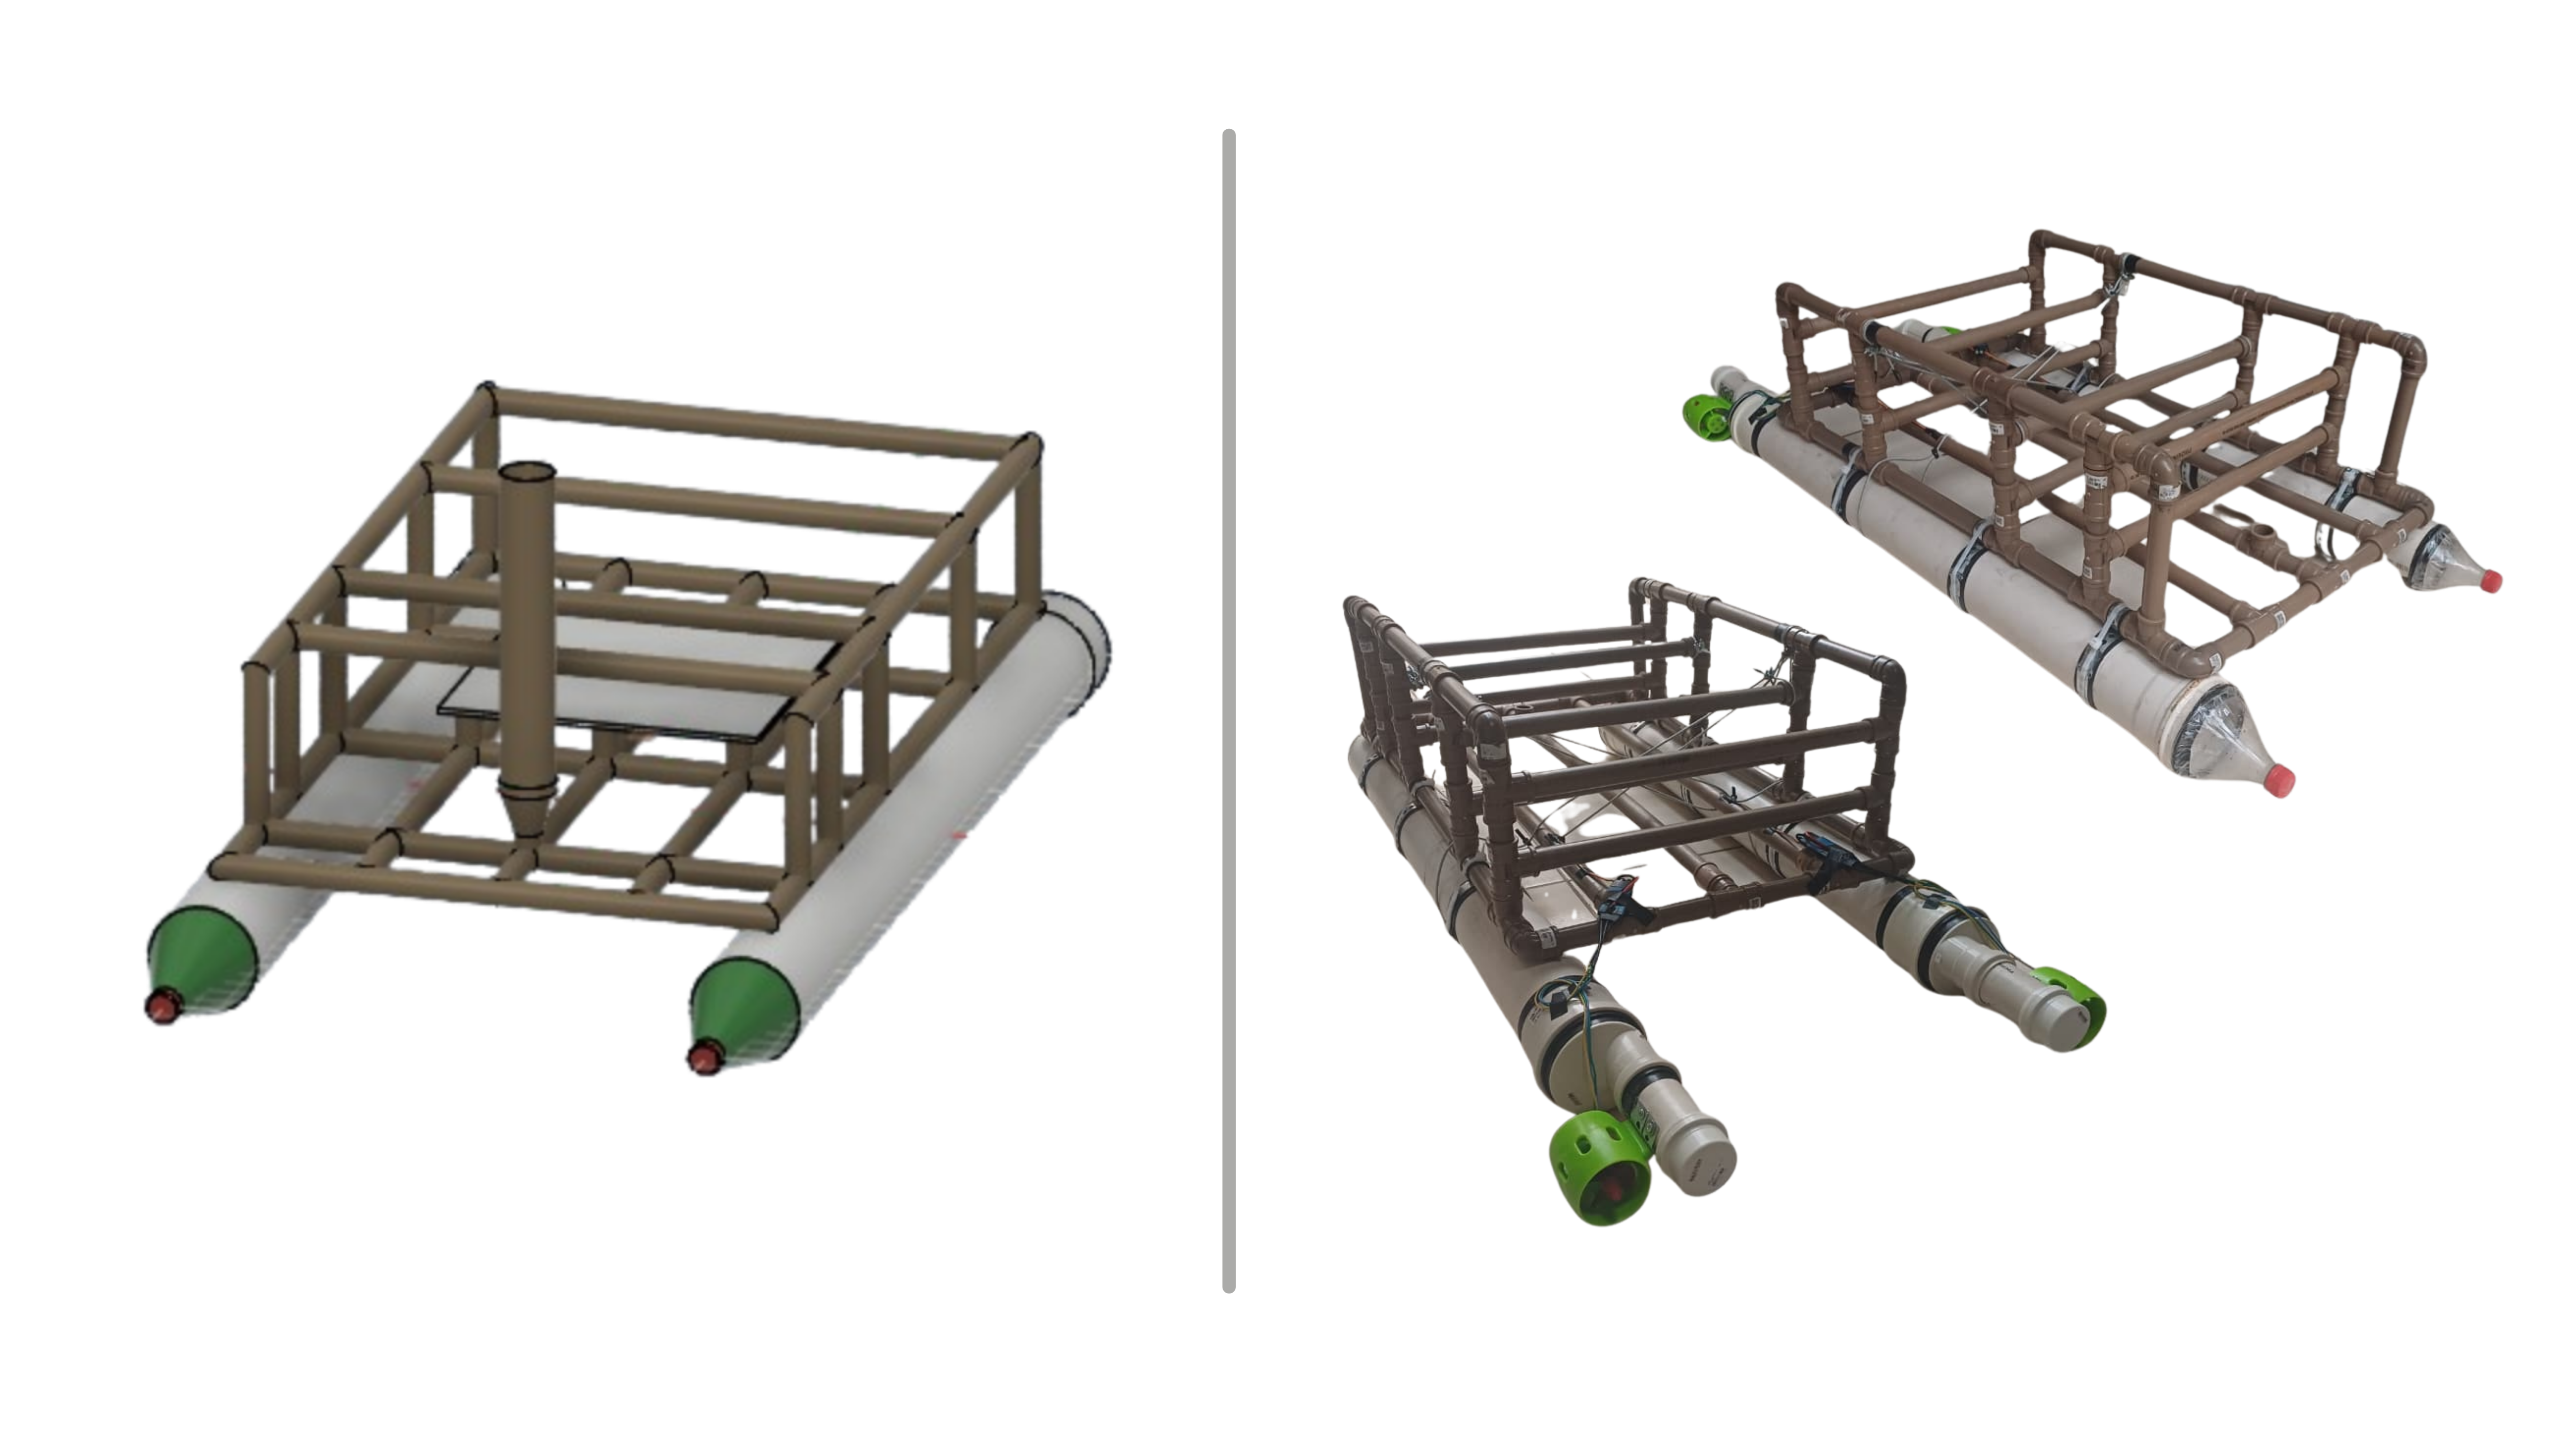
\includegraphics[width=0.7\textwidth]{estrutura_comparativo.png}
\caption{Comparativo entre o modelo CAD 3D e a estrutura física do catamarã em PVC com motores e ESCs integrados.}
\label{fig:evidencia_estrutura}
\end{figure}


\subsubsection{Prototipagem Eletrônica}

O ESP32 e o módulo A7670SA foram integrados inicialmente em protoboard para validação de níveis lógicos e estabilidade de alimentação. A Figura \ref{fig:evidencia_eletronica} ilustra a bancada de testes.

\begin{figure}[H]
\centering
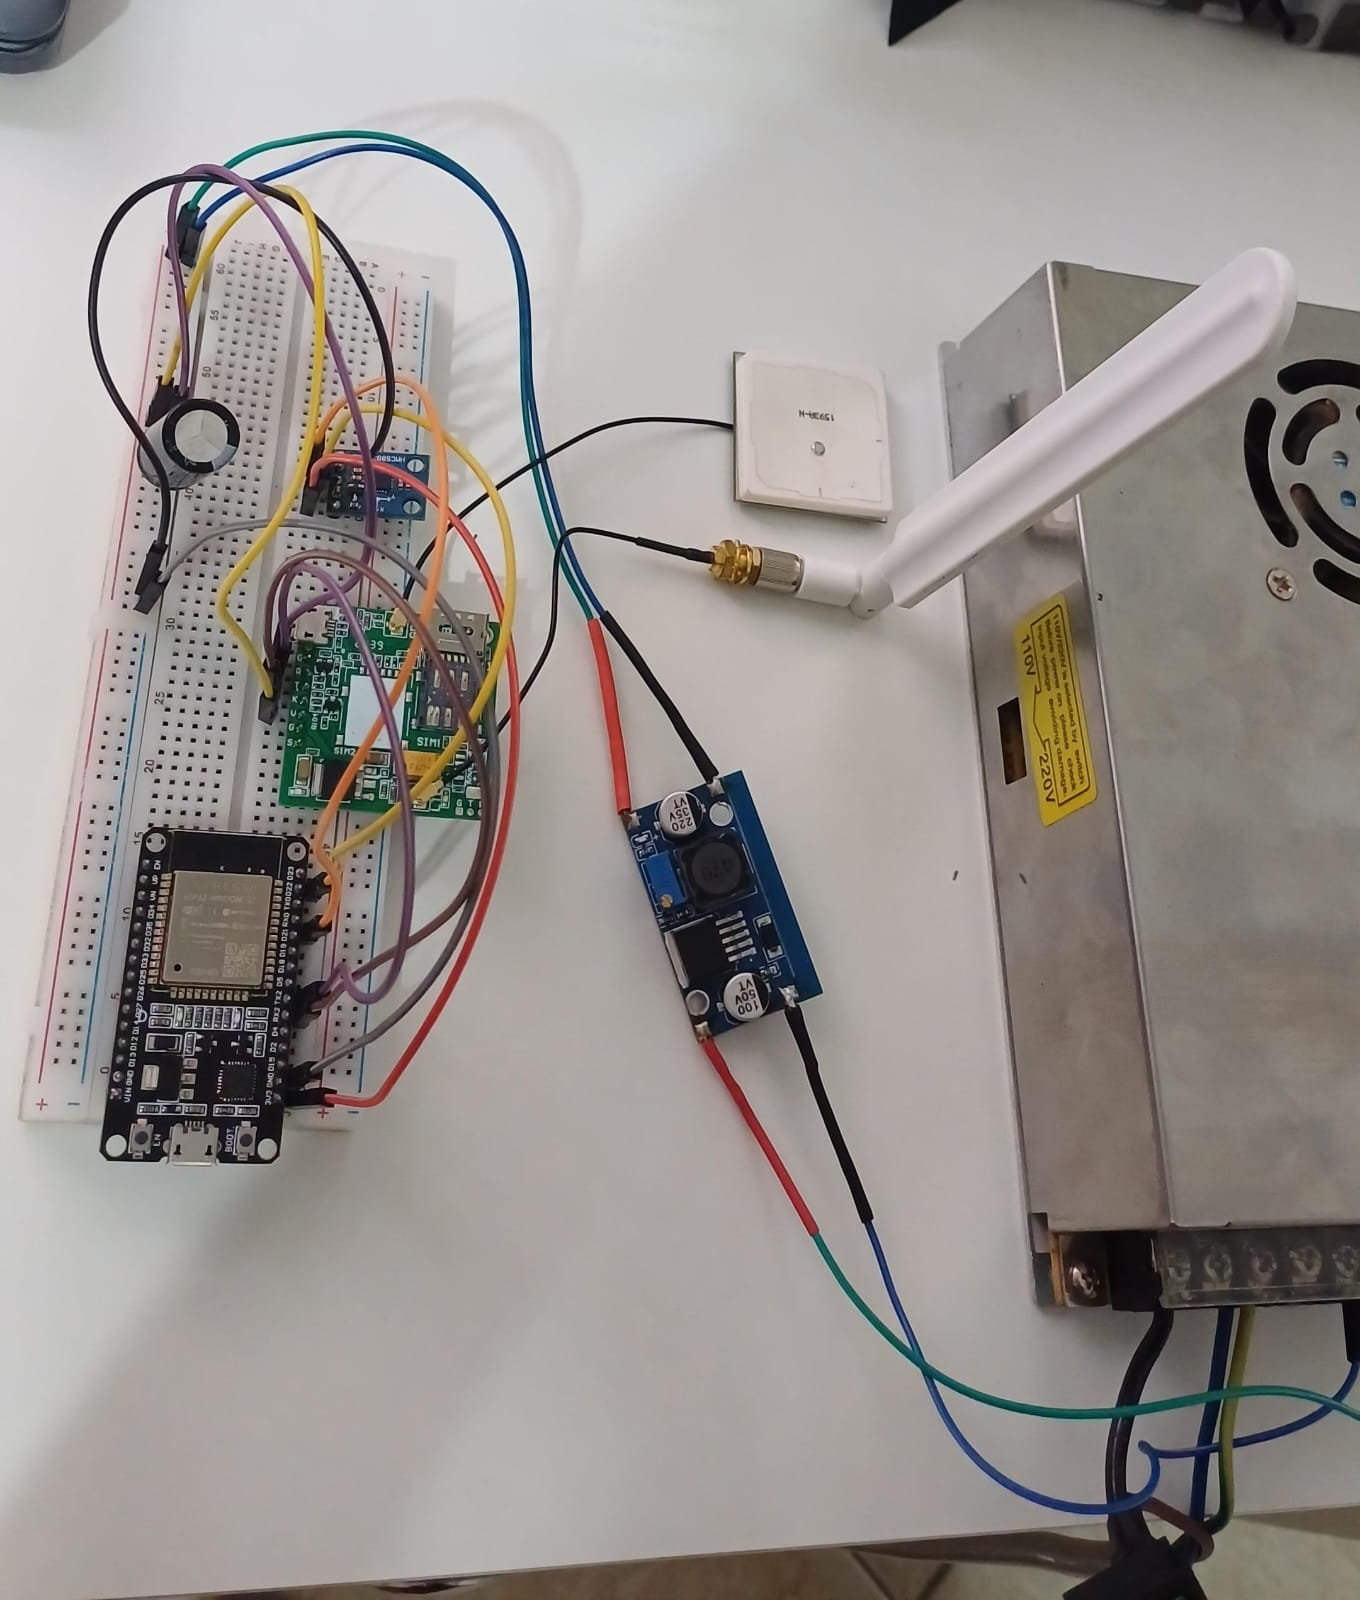
\includegraphics[width=0.4\textwidth]{prototipagem_eletronica.jpg}
\caption{Montagem em protoboard: ESP32, módulo 4G, sensores e circuito de nível lógico.}
\label{fig:evidencia_eletronica}
\end{figure}

\begin{figure}[H]
\centering
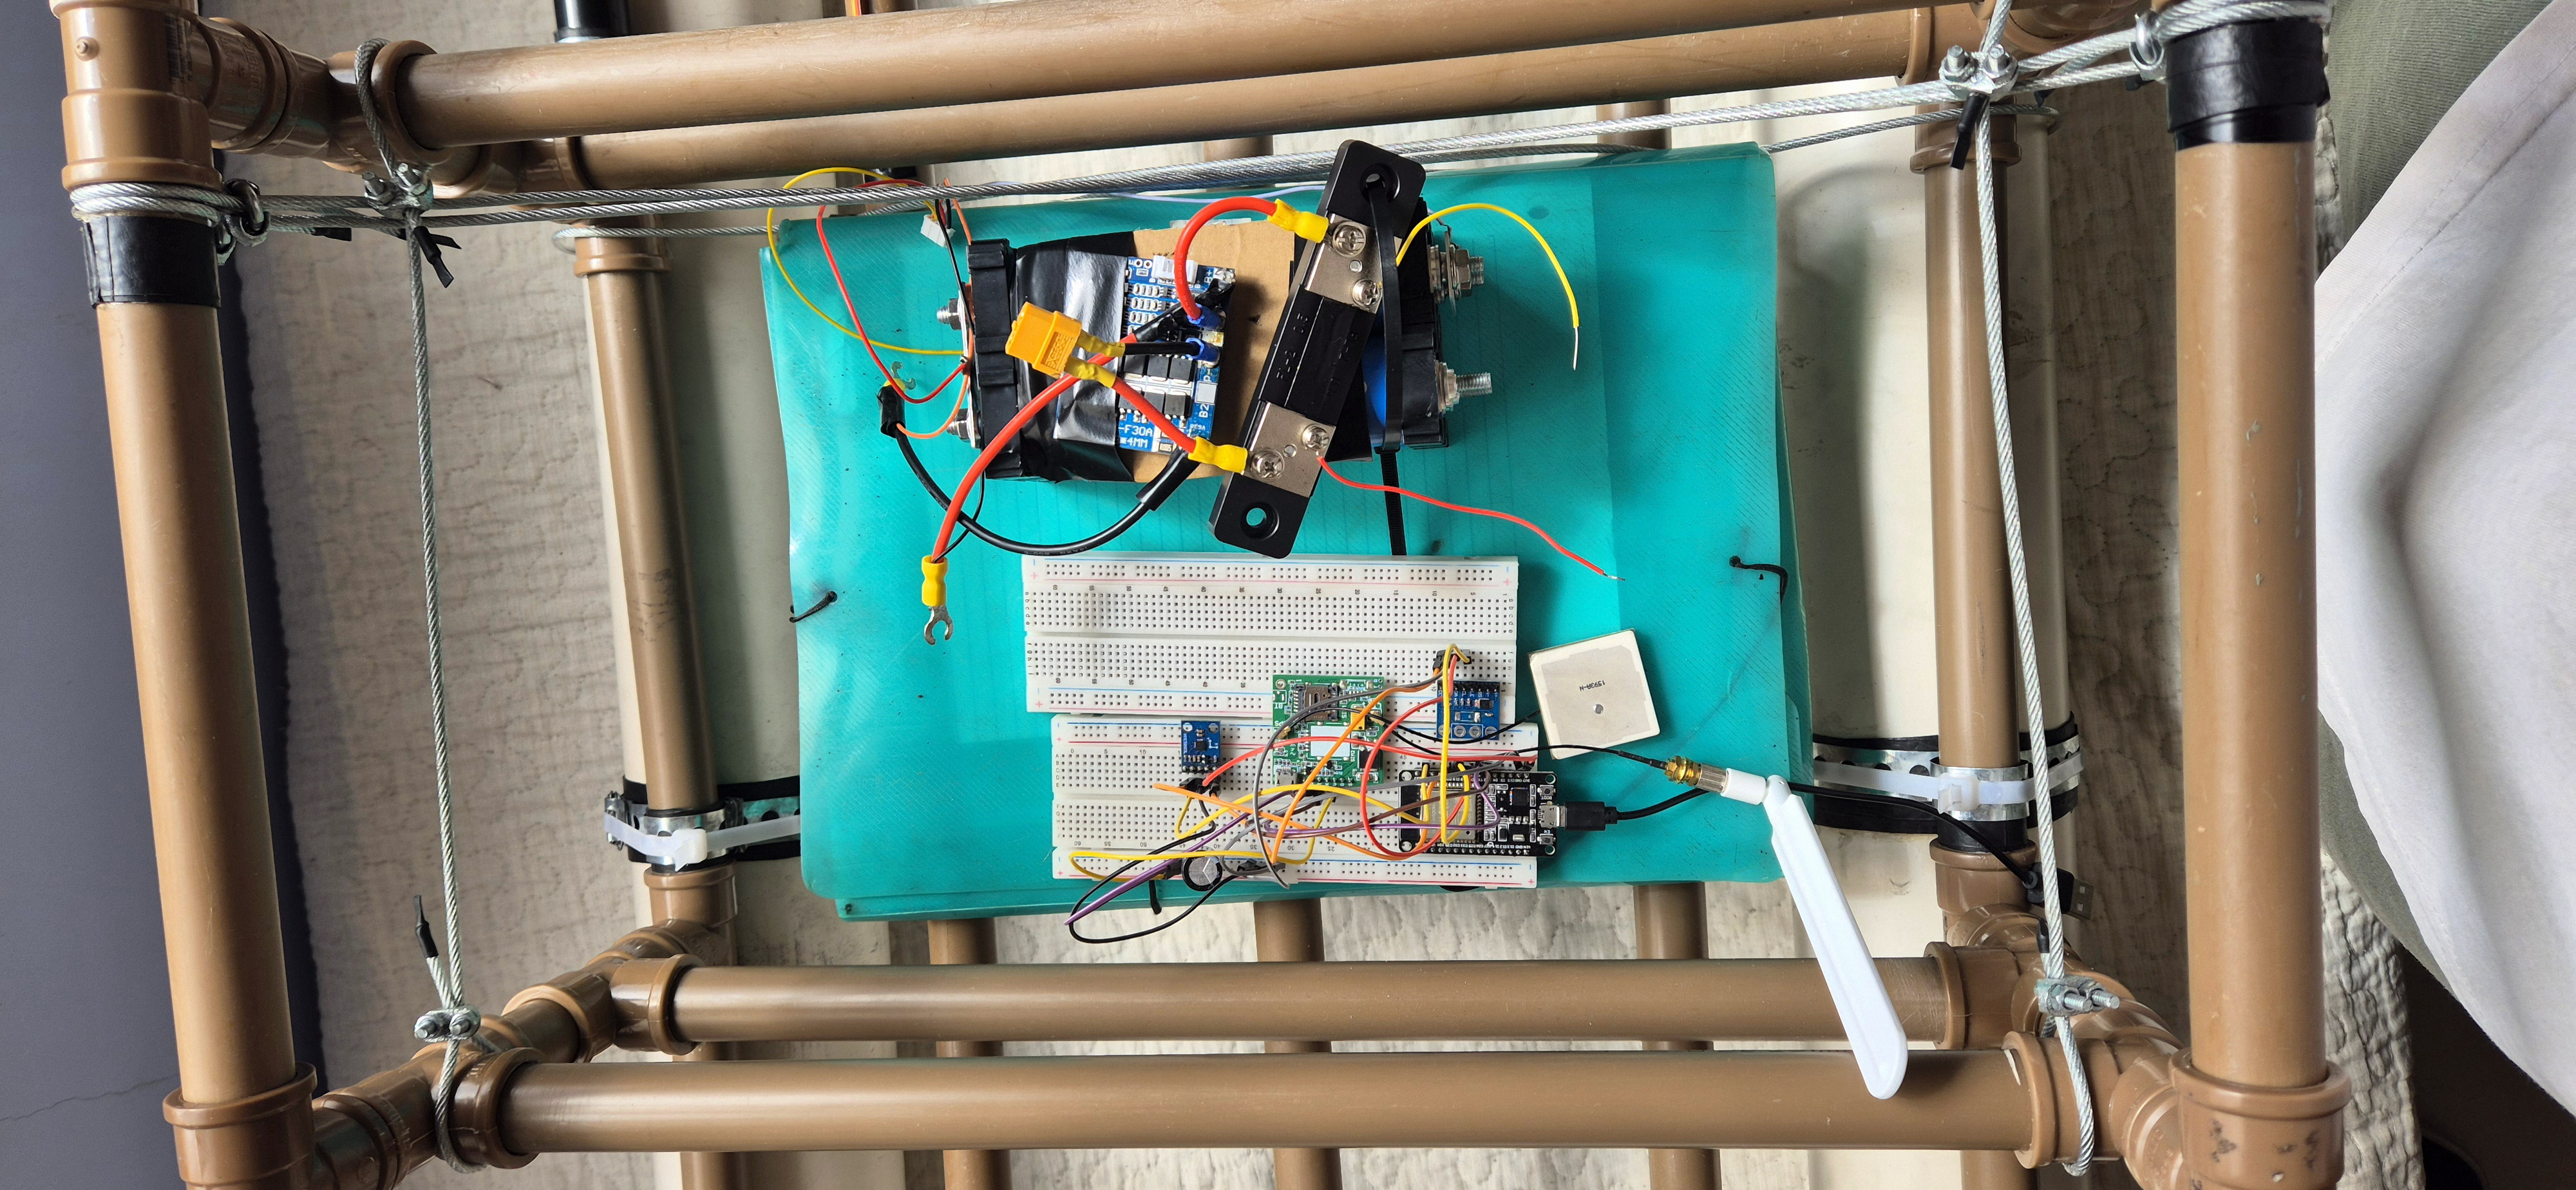
\includegraphics[width=0.4\textwidth]{BMSBattery.jpg}
\caption{Sistema de processamento central em processo de integração com a BMS + Bateria}
\label{fig:BMS}
\end{figure}

\subsection{Teste de Flutuabilidade}

O catamarã foi submetido a ensaio hidrostático em piscina controlada. O veículo flutuou com equilíbrio satisfatório, sem inclinação perceptível, validando a distribuição de massa e a reserva de flutuabilidade dos cascos de PVC com proas PET. A reserva estimada com a massa atual (sem os flutuadores de EVA) é de 31{,}3\%, acima do limite crítico de operação, mas abaixo da meta de projeto de 40\%. A implementação dos flutuadores de EVA (``macarrão de piscina'') está prevista para ampliar essa margem para 65{,}3\%.

\begin{figure}[H]
\centering
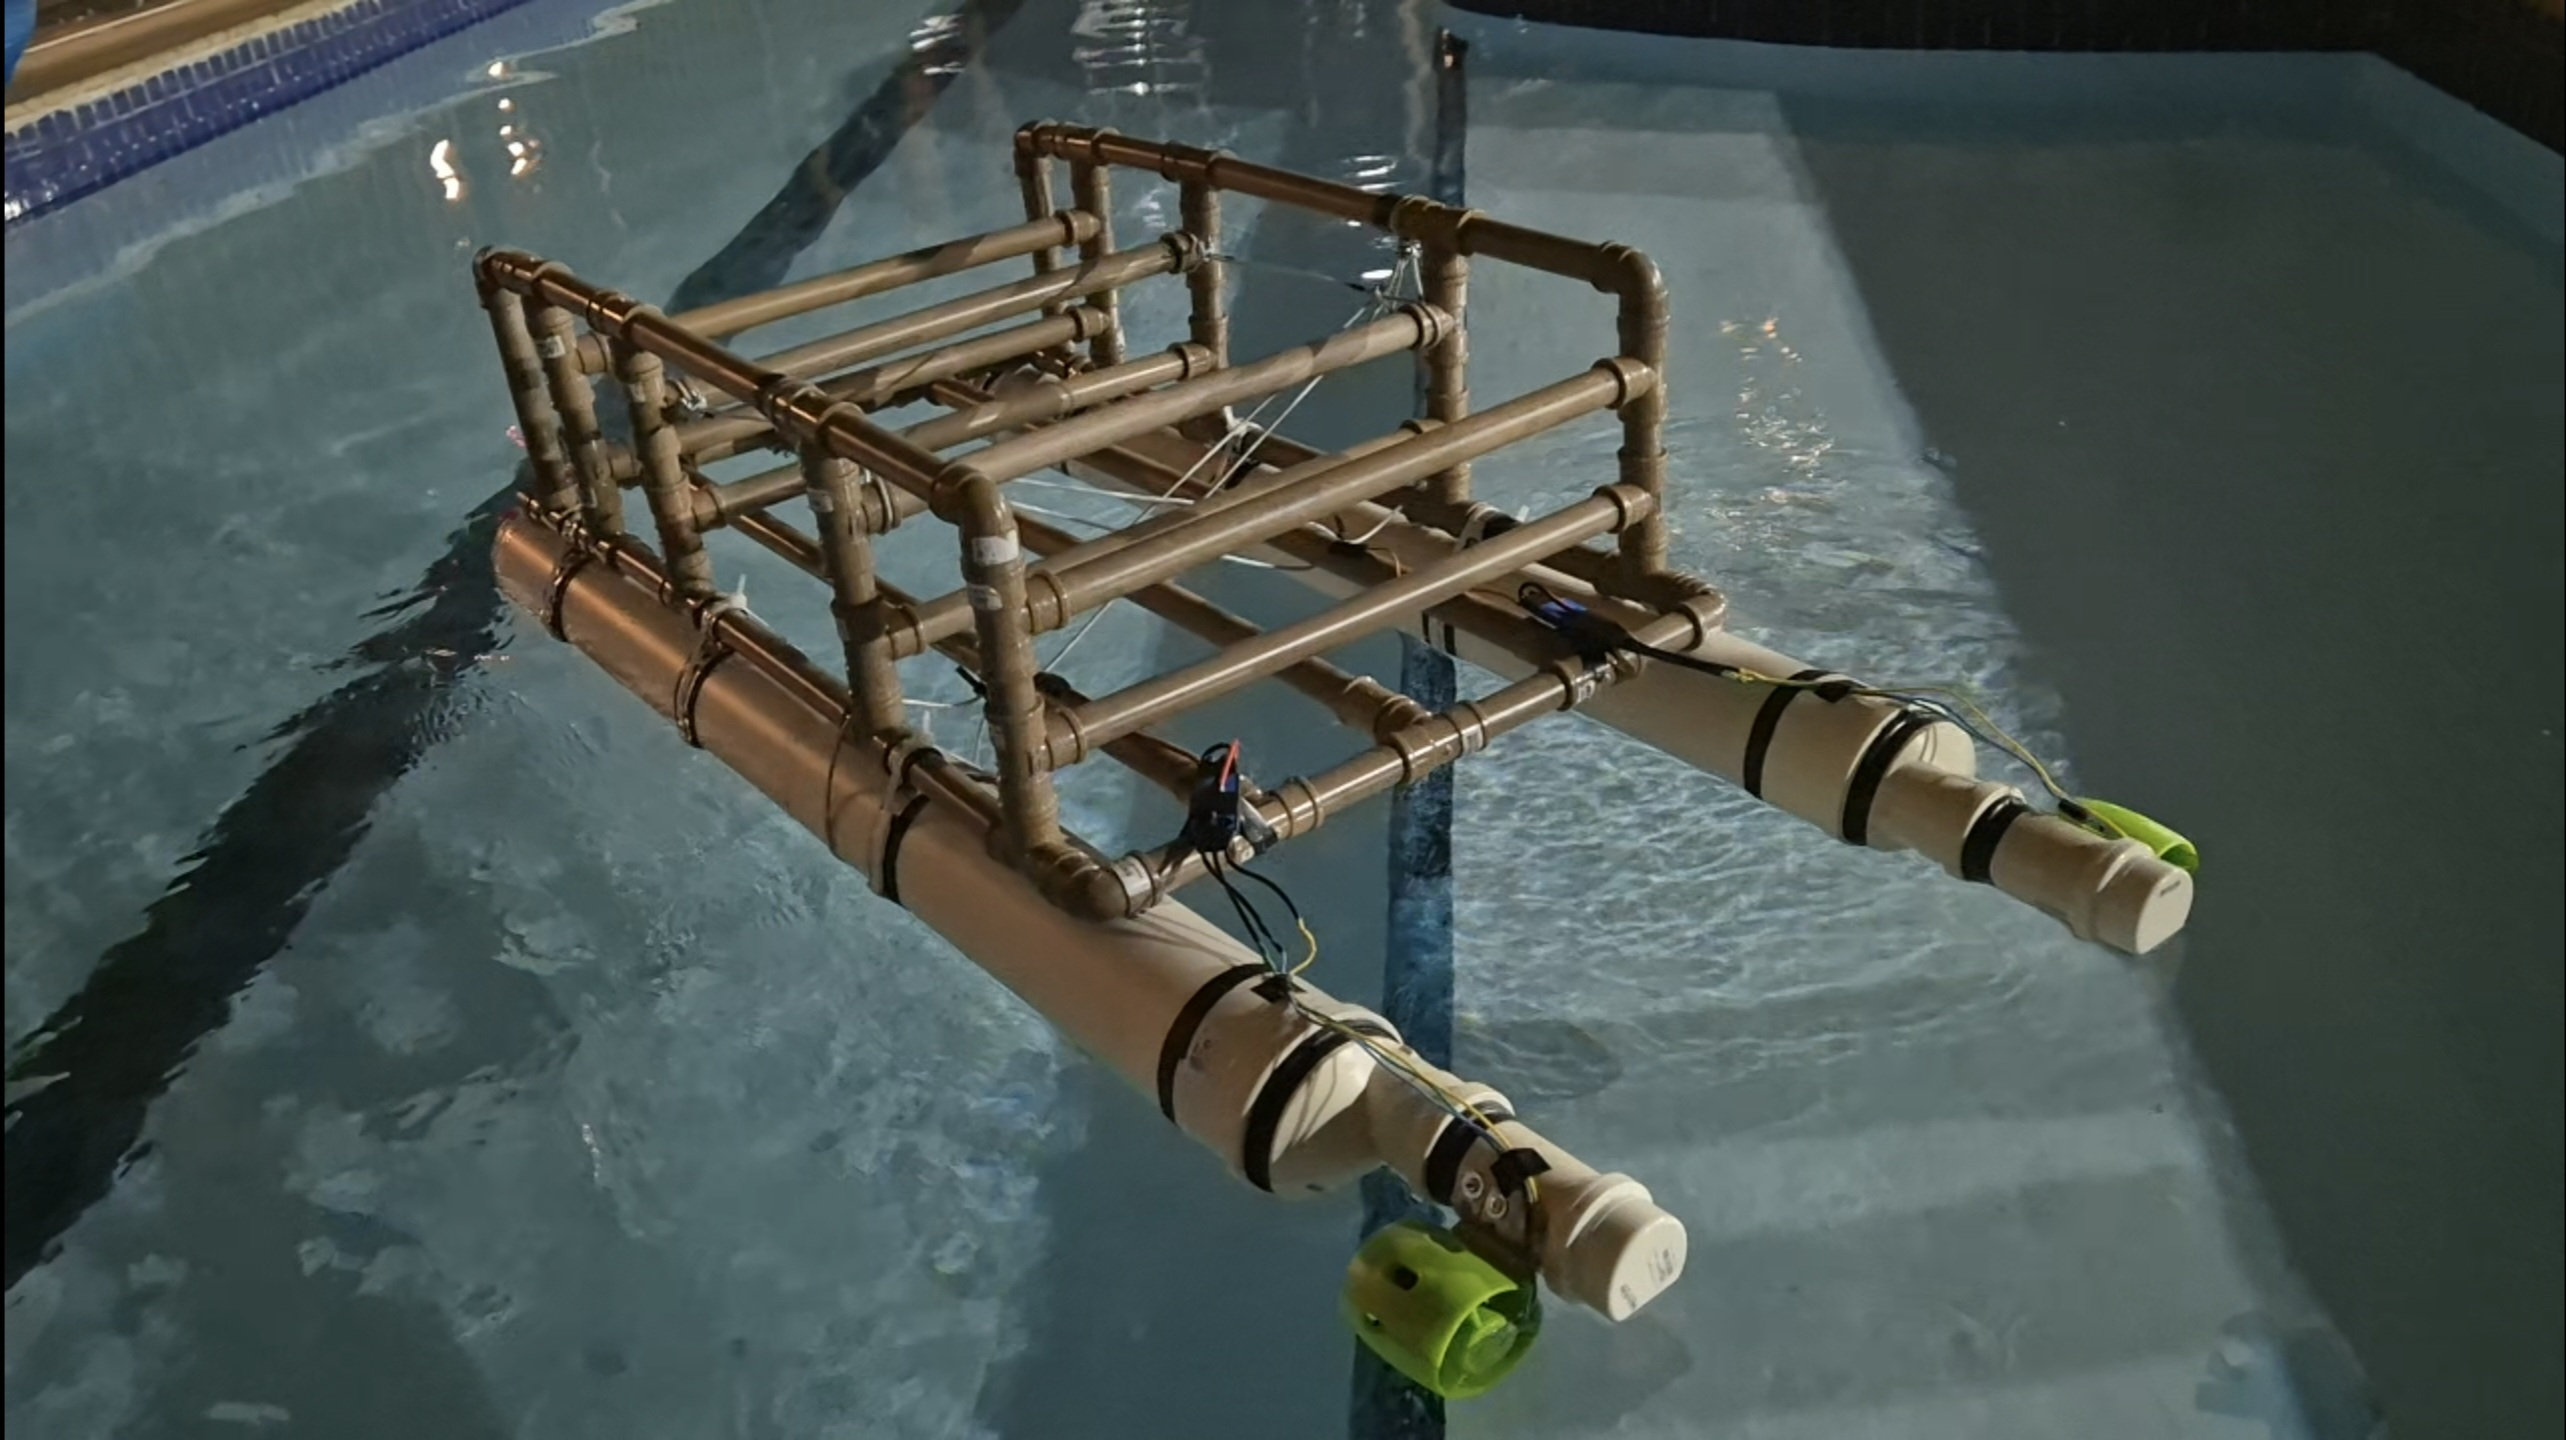
\includegraphics[width=0.4\textwidth]{Flutuabilidade.jpg}
\caption{Testes de flutuabilidade com os motores integrados à estrutura física.}
\label{fig:flutuabilidade}
\end{figure}

\subsection{Integração dos Motores e ESCs}

Os motores BLDC e os ESCs foram fixados fisicamente à estrutura do catamarã. Nesta etapa, os motores ainda não foram acionados em propulsão no ambiente aquático, a integração foi mecânica e elétrica. O cabeamento entre os ESCs e os motores percorre os cascos externamente, encapsulado em fita isolante para proteção mecânica e impermeabilização parcial.

\subsection{Testes de Componentes em Bancada}

\textbf{Bateria + BMS:} A arquitetura de conexões entre o \textit{pack} LiFePO4 e o módulo BMS-4S foi estabelecida. Foram realizados testes básicos de estabilidade do conjunto.

\begin{figure}[H]
\centering
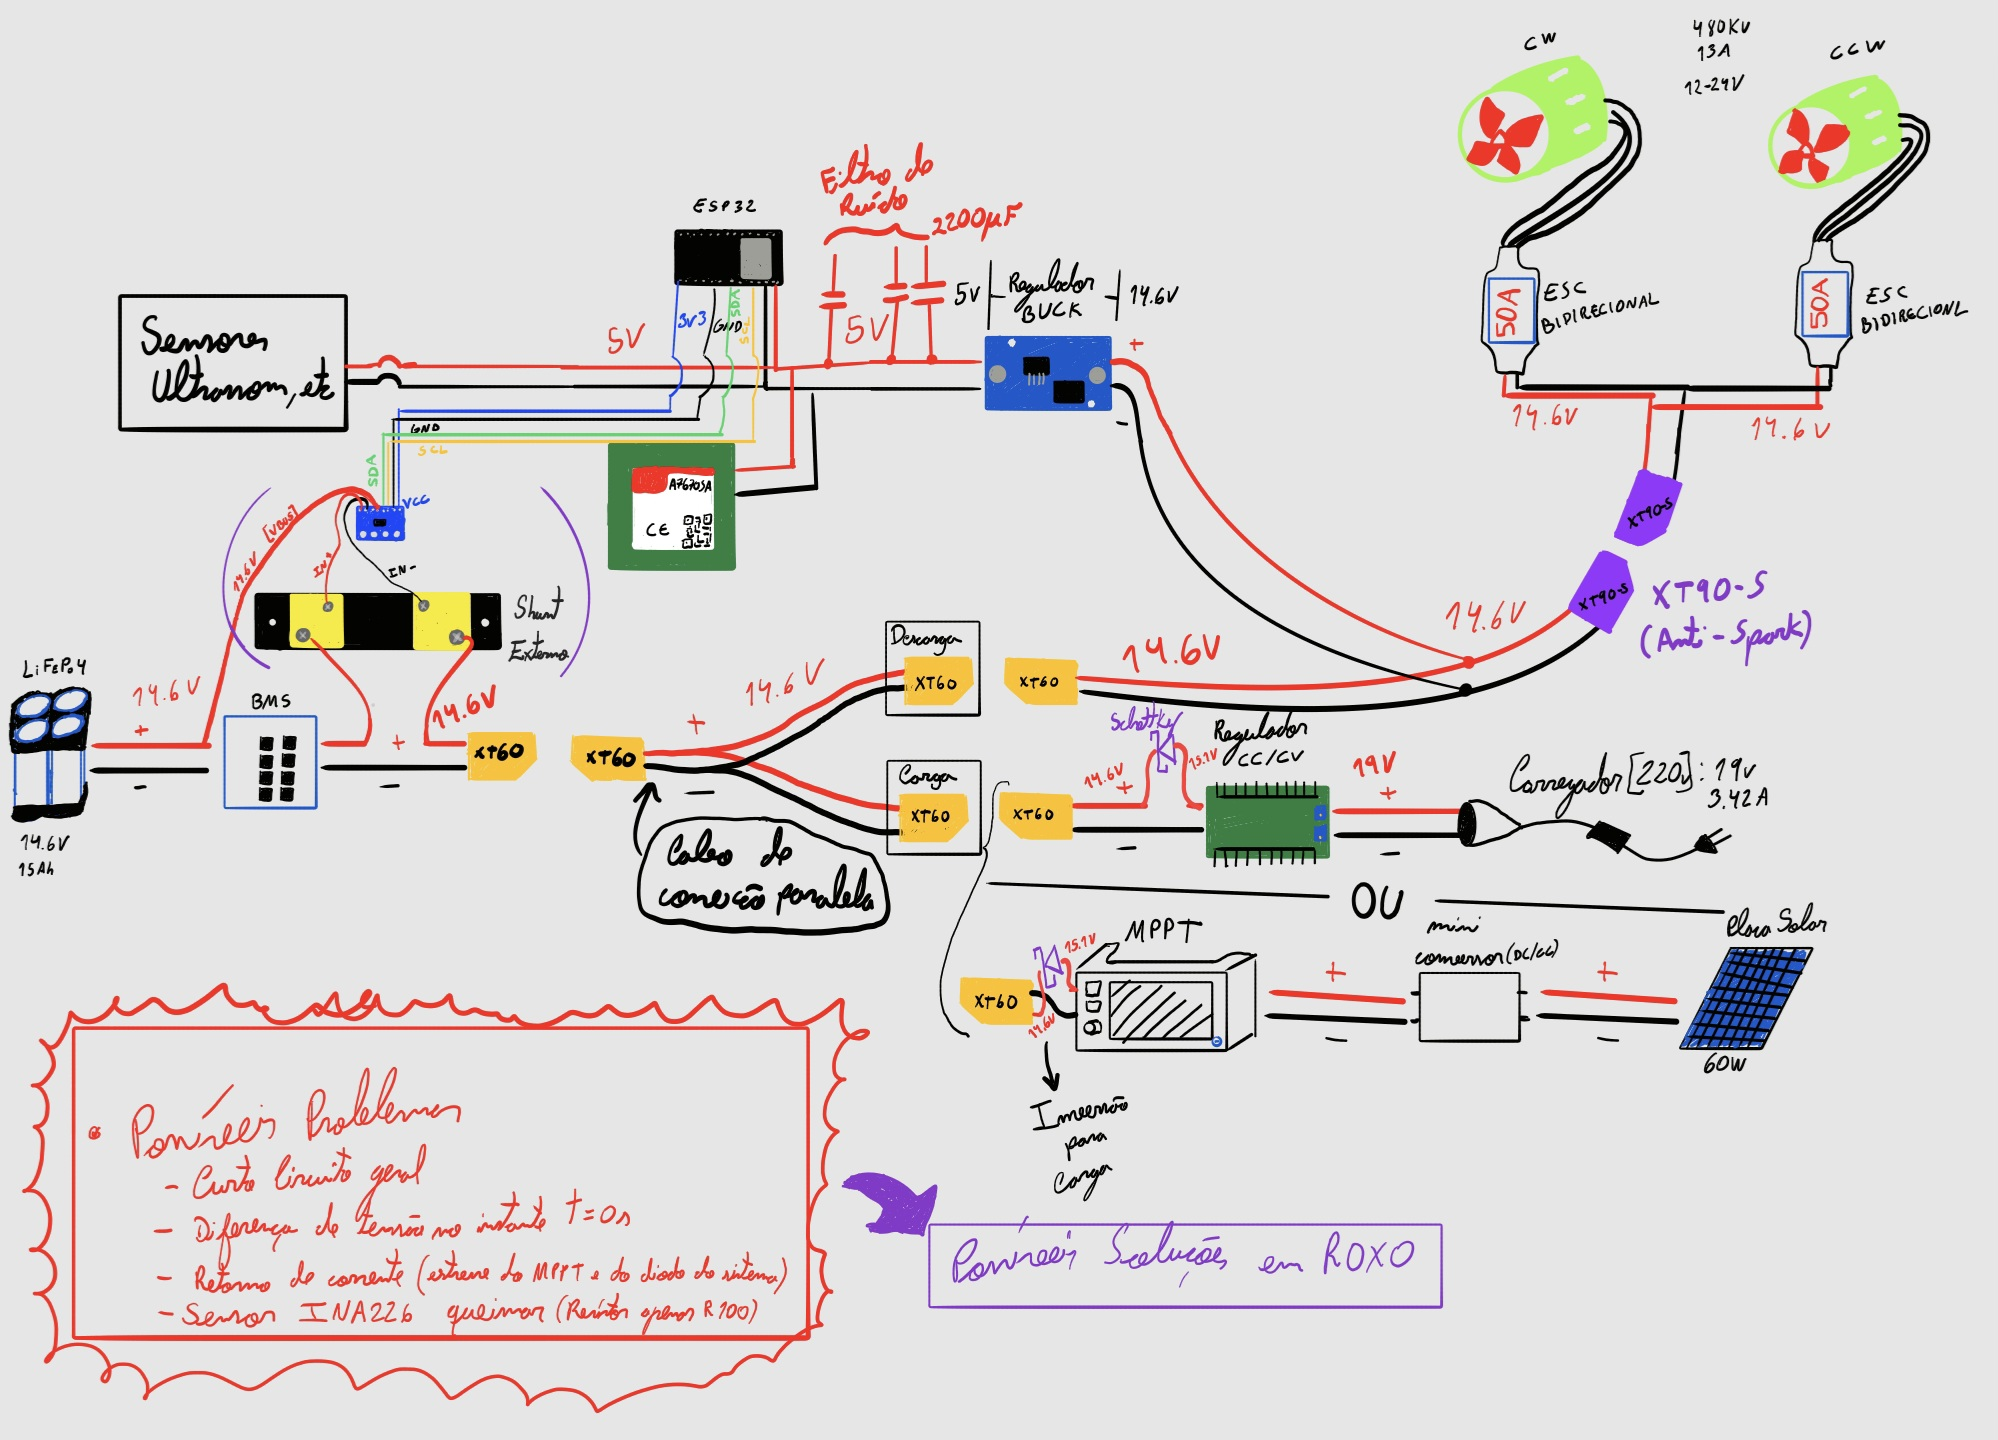
\includegraphics[width=0.7\textwidth]{DiagramaAlimentacao.jpg}
\caption{Diagrama total realizado para melhor representação e resolução de problemas}
\label{fig:diagrama_alimentacao}
\end{figure}

\textbf{Motores com a bateria do projeto:} Os motores foram acionados diretamente pela bateria LiFePO4 via ESCs, confirmando compatibilidade elétrica do sistema de propulsão. Foi proposto, nesse primeiro momento, um firmware mínimo de acionamento dos motores.

% ------------------------------------------------------------------
\subsubsection{Detalhamento do Sistema Elétrico de Propulsão}

\paragraph{Arquitetura do Barramento:}
A distribuição de energia opera a partir de um banco LiFePO4 4S (15~Ah, 14,6~V de pico) gerenciado pelo BMS e divide-se em dois ramais fisicamente separados: o \textbf{ramal lógico}, que alimenta a ESP32 e periféricos via conversor Buck (5~V), e o \textbf{ramal de tração}, que alimenta os dois ESCs bidirecionais de 50~A. Essa separação é essencial porque os capacitores de entrada dos ESCs (até 2000~$\mu$F) geram correntes de \textit{inrush} elevadíssimas em $t = 0$~s, enquanto o Buck da lógica opera com capacitores de 10--47~$\mu$F, cujo transiente é desprezível.

\begin{figure}[H]
\centering
\includegraphics[width=0.65\textwidth]{topologia-conexoes-2.png}
\caption{Topologia do barramento de potência: bateria LiFePO4, BMS, ramais lógico e de tração.}
\label{fig:topologia1}
\end{figure}

\paragraph{Proteções Implementadas:}
A análise da topologia inicial revelou quatro vulnerabilidades críticas, cada uma endereçada com um componente ou decisão de projeto específica:

\begin{itemize}
\item \textbf{\textit{Inrush Current} (faísca no engate):} Adoção do conector XT90-S (\textit{Anti-Spark}) no ramal de tração. Seu resistor interno de 5,6~$\Omega$ pré-carrega suavemente os capacitores dos ESCs antes de estabelecer a conexão de baixa impedância, eliminando o arco voltaico.

\item \textbf{Retorno de Corrente (\textit{Backfeeding}):} Instalação de diodos Schottky (10SQ050, 10~A/50~V) nos cabos positivos de cada fonte de carga (MPPT e fonte de parede). Atuam como válvulas de retenção: permitem que as fontes carreguem a bateria, mas bloqueiam qualquer corrente reversa quando estão inativas. A queda de $\approx 0,5$~V do diodo é compensada calibrando a saída das fontes para 15,1~V.

\item \textbf{Queima do Sensor de Corrente:} O resistor SMD original da placa INA226 (R100) foi removido e substituído por um \textit{shunt} externo de metal maciço (50~A / 75~mV) inserido diretamente no cabo de tração, eliminando a limitação térmica do componente original.

\item \textbf{Inviabilidade de Chaveamento Manual:} A porta de carga foi unificada em um único conector XT60. Como os carregadores (painel solar e tomada) operam em ambientes mutuamente excludentes — água e bancada, respectivamente — compartilham a mesma entrada sem necessidade de chave seletora, preservando a autonomia do ASV.
\end{itemize}

\begin{figure}[H]
\centering
\includegraphics[width=0.65\textwidth]{topologia-escs.png}
\caption{Detalhe das conexões dos ESCs bidirecionais.}
\label{fig:topologia2}
\end{figure}

\paragraph{Telemetria Energética (INA226).}
Com o \textit{shunt} externo instalado, o chip INA226 opera como um coprocessador de energia dedicado: seu ADC interno de 16~bits mede a micro-queda de tensão no manganim e entrega, via I2C, os valores de tensão, corrente e potência diretamente em registradores nativos. Isso poupa processamento da ESP32 e oferece imunidade quase absoluta ao ruído eletromagnético gerado pelos motores.

% ------------------------------------------------------------------
\subsubsection{Firmware de Controle: Arquitetura e Algoritmos}

O código-fonte completo está disponível no repositório: \url{https://github.com/AlphaCompLabs/H-Drop/tree/main/Motors-Simulation}.

O \textit{firmware} de validação dos motores em bancada transforma a ESP32 em um servidor HTTP embarcado, dispensando aplicativos de terceiros ou Bluetooth --- que apresentam alcance limitado em ambientes aquáticos. O celular do operador funciona simultaneamente como roteador (Hotspot Wi-Fi) e cliente (navegador web), enquanto a ESP32 atua como dispositivo conectado (\textit{station}) e servidor.

\paragraph{Backend (C++ na ESP32):} O núcleo do \textit{firmware} gerencia três responsabilidades simultâneas. A primeira é a alocação de hardware com PWM preciso: a biblioteca \texttt{ESP32Servo} é vinculada a \textit{Hardware Timers} dedicados do chip, garantindo que a modulação por largura de pulso (PWM a 50~Hz) mantenha estabilidade mesmo durante o processamento das requisições HTTP. A segunda é o roteamento HTTP com API RESTful simplificada, exposta na porta 80. A terceira é a sequência de armamento dos ESCs (\textit{Arming Sequence}), descrita a seguir.

O trecho abaixo ilustra a alocação dos timers e o procedimento de armamento, que envia o sinal de ponto morto (1520~$\mu$s) por 4 segundos antes de habilitar o servidor para recebimento de comandos:

\begin{lstlisting}[language=C++, caption={Alocação de timers e sequência de armamento dos ESCs (setup).}, label=lst:arming]
ESP32PWM::allocateTimer(0);
ESP32PWM::allocateTimer(1);
escEsquerdo.setPeriodHertz(50);
escDireito.setPeriodHertz(50);
escEsquerdo.attach(pinoESCEsquerdo, 1000, 2000);
escDireito.attach(pinoESCDireito, 1000, 2000);

// Envia 1520us para armar os ESCs corretamente
escEsquerdo.writeMicroseconds(PONTO_MORTO);
escDireito.writeMicroseconds(PONTO_MORTO);
delay(4000);
\end{lstlisting}

O roteamento HTTP define \textit{endpoints} para controle individual e em lote. O \textit{endpoint} \texttt{/motor} aceita parâmetros dinâmicos (\texttt{?lado=E\&pwm=1650}), viabilizando controle granular de cada propulsor. Os \textit{endpoints} \texttt{/frente}, \texttt{/re} e \texttt{/parar} disparam comandos predefinidos para ambos os motores simultaneamente:

\begin{lstlisting}[language=C++, caption={Rota de controle individual por motor via parâmetros HTTP.}, label=lst:rota_motor]
server.on("/motor", []() {
  if (server.hasArg("lado") && server.hasArg("pwm")) {
    String lado = server.arg("lado");
    int pwm = server.arg("pwm").toInt();
    if (lado == "E") escEsquerdo.writeMicroseconds(pwm);
    if (lado == "D") escDireito.writeMicroseconds(pwm);
    server.send(200, "text/plain", "OK");
  }
});

server.on("/parar", []() {
  escEsquerdo.writeMicroseconds(PONTO_MORTO);
  escDireito.writeMicroseconds(PONTO_MORTO);
  server.send(200, "text/plain", "OK");
});
\end{lstlisting}

O \textit{fail-safe} de atualização OTA (\textit{Over-The-Air}) é outro mecanismo de segurança relevante: ao iniciar o carregamento de um novo \textit{firmware} via rede durante a navegação, o evento \texttt{ArduinoOTA.onStart()} aplica imediatamente o sinal de 1520~$\mu$s (PARAR) aos ESCs, colocando a embarcação em estado de deriva segura durante o ciclo de atualização.

\paragraph{Frontend (Interface Móvel):} A interface visual é armazenada diretamente na memória \textit{flash} da ESP32 via diretiva \texttt{PROGMEM} e formatação \texttt{R"rawliteral(...)rawliteral"}, dispensando sistemas de armazenamento externos. O layout é responsivo (\textit{Mobile-First}), com botões e \textit{sliders} dimensionados para telas de dispositivos móveis. O controle em tempo real é implementado com requisições assíncronas JavaScript (\texttt{fetch()}): ao mover um \textit{slider}, o evento \texttt{oninput} dispara a transmissão da requisição HTTP em segundo plano, sem recarregar a página, refletindo as interações nos motores com latência mínima. A sincronização lógico-visual garante que botões de estado absoluto (como ``PARAR'' ou ``FRENTE'') atualizem simultaneamente o estado real do hardware e a representação gráfica dos \textit{sliders} na interface.

\begin{figure}[H]
\centering
\includegraphics[width=0.30\textwidth]{tela-app.jpeg}
\caption{Interface de controle servida diretamente pela ESP32 e acessada via navegador no celular.}
\label{fig:tela_app}
\end{figure}

\paragraph{Zona Morta dos ESCs (\textit{Deadband}).} Um comportamento técnico relevante identificado nos ESCs é a presença de uma banda morta em torno do ponto neutro calibrado de 1520~$\mu$s. A rampa de aceleração não se inicia linearmente em 1521~$\mu$s: existe uma tolerância de histerese estimada em $\pm 100$~$\mu$s. Essa banda morta protege o sistema contra oscilações de sinal residuais, comuns em transmissores com retorno por mola, que causariam acionamento oscilatório dos motores em repouso. Para a futura implementação do controlador PID autônomo, essa característica exigirá um Compensador de \textit{Deadband} (\textit{piecewise function}): quando a malha de controle exigir empuxo mínimo positivo, o processador deve aplicar um \textit{offset} de 100~$\mu$s, saltando diretamente para 1620~$\mu$s, evitando que comandos de correção leve incidam na zona de corte de potência e acumulem indevidamente o termo integral do erro.

% ------------------------------------------------------------------
\subsubsection{Envelope de Potência e Parâmetros Operacionais}

A Tabela~\ref{tab:envelope_pwm} consolida os parâmetros de comando PWM do sistema de propulsão, com base na caracterização empírica dos ESCs em bancada.

\begin{table}[H]
\centering
\caption{Envelope de potência e zonas de operação dos ESCs bidirecionais de 50~A}
\label{tab:envelope_pwm}
\renewcommand{\arraystretch}{1.3}
\begin{tabularx}{\textwidth}{|c|c|c|X|}
\hline
\rowcolor{gray!20}
\textbf{Zona} & \textbf{Faixa de PWM ($\mu$s)} & \textbf{Estado do Motor} & \textbf{Observação} \\ \hline
Tração Positiva & 1620 -- 2000 & Avanço crescente & Limiar efetivo após \textit{deadband} \\ \hline
\rowcolor{gray!10}
Zona Morta & 1420 -- 1620 & Corte de potência & Repouso absoluto; protege contra ruído de sinal \\ \hline
Tração Negativa & 1000 -- 1420 & Ré crescente & Limiar efetivo após \textit{deadband} \\ \hline
\rowcolor{gray!10}
Ponto Morto (Arming) & 1520 & Neutro calibrado & Sinal de referência enviado por 4~s no boot \\ \hline
Frente (Padrão) & 1600 & Avanço suave & Comando do botão ``FRENTE'' da interface \\ \hline
\rowcolor{gray!10}
Ré (Padrão) & 1400 & Ré suave & Comando do botão ``RÉ'' da interface \\ \hline
\end{tabularx}
\end{table}

% ------------------------------------------------------------------
\subsubsection{Vídeo de Validação em Bancada}

O vídeo a seguir demonstra o acionamento dos motores em bancada, com controle via interface web, confirmando a resposta dos ESCs aos comandos de avanço, ré e parada de emergência:

\begin{center}
\textbf{Link do vídeo 1:} {\color{blue} [https://photos.app.goo.gl/3MceCbJM5Kov54rX7]}
\end{center}


\noindent A gravação evidencia o funcionamento coordenado dos dois propulsores, a responsividade da interface \textit{Mobile-First} e a estabilidade do sinal PWM gerado pelos \textit{Hardware Timers} da ESP32 durante o processamento simultâneo das requisições HTTP.


% ------------------------------------------------------------------


\subsection{Sistema de Simulação de Controle Embarcado}

Com a integração elétrica dos motores concluída apenas nas etapas finais do PC3, o desenvolvimento do algoritmo de controle não poderia esperar a disponibilidade do hardware completo. Para isso, foi desenvolvido um ambiente de simulação em três camadas, \textit{firmware} real na ESP32, servidor Python e \textit{dashboard} web, capaz de exercitar todas as variáveis do sistema de forma integrada, validando a lógica de navegação antes dos ensaios aquáticos.

\begin{figure}[H]
\centering
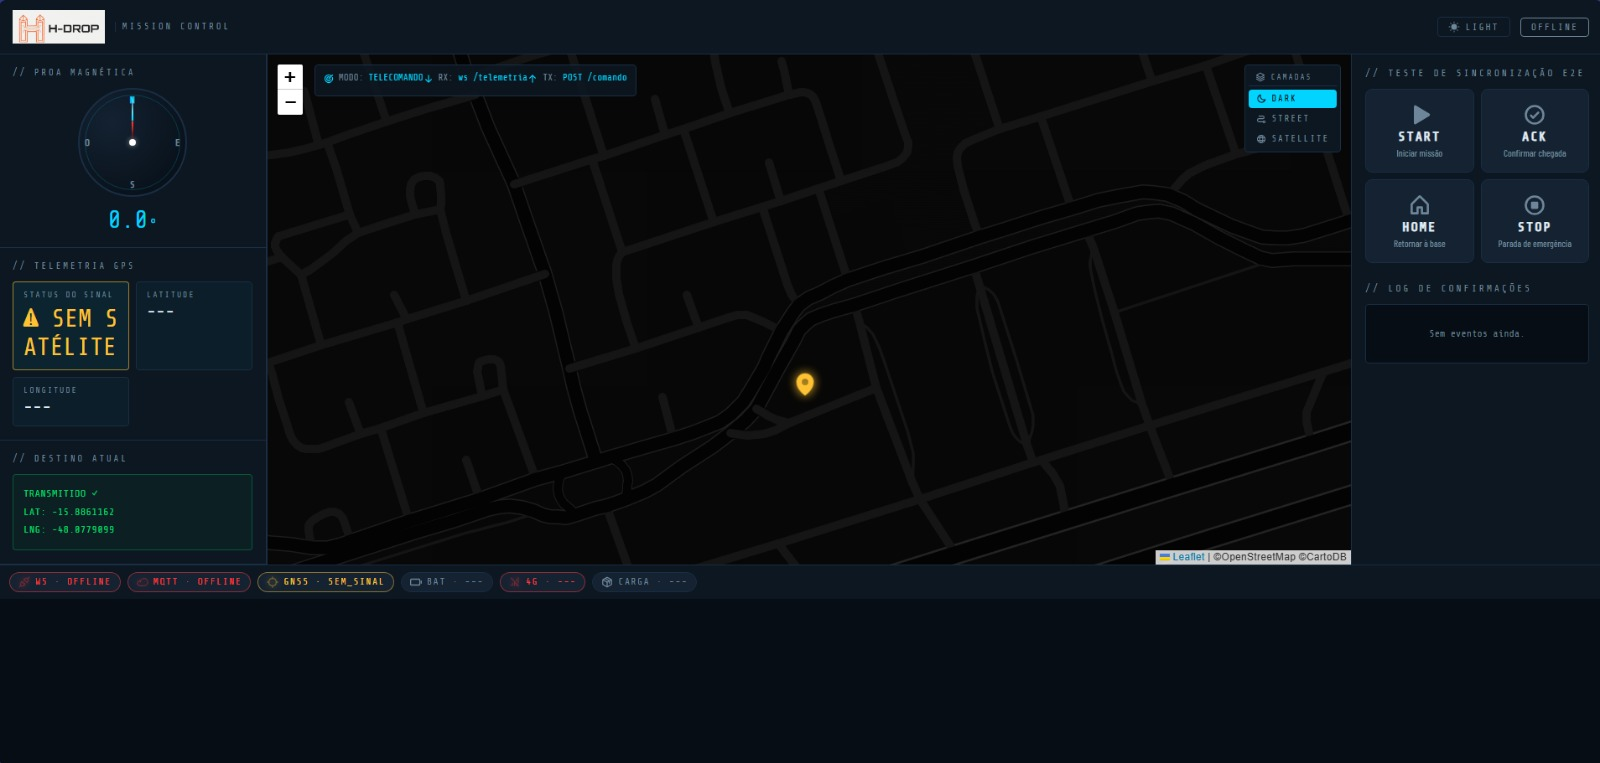
\includegraphics[width=0.65\textwidth]{print-dashboard-completo.png}
\caption{\textit{Dashboard} HDrop: visão geral do sistema de simulação com telemetria em tempo real.}
\label{fig:dashboard_geral}
\end{figure}

% ------------------------------------------------------------------
\subsubsection{Arquitetura do Ambiente de Simulação}

O código-fonte completo está disponível no repositório: \url{https://github.com/AlphaCompLabs/H-Drop/tree/main/Controler-Simulation}.
O ambiente é composto por três componentes independentes que se comunicam entre si:

\begin{itemize}
\item \textbf{Firmware (\texttt{main.c} — ESP32):} Código C real rodando no microcontrolador com FreeRTOS. Implementa a máquina de estados, os controladores PD/PI, a lógica de missão e o pipeline de sensores. Sensores fisicamente ausentes (INA226 e AJ-SR04M) são substituídos por funções de simulação internas (\texttt{bat\_simular()} e \texttt{us\_ler\_simulado()}).
\item \textbf{Servidor Python (\texttt{hdrop\_sim.py}):} Simula o barco inteiro — GNSS, magnetômetro, ultrassônico, bateria e controle PD — e serve o \textit{dashboard} via HTTP na porta 5000. Opera, por enquanto, de forma independente do firmware, permitindo visualização durante o desenvolvimento sem hardware conectado.
\item \textbf{Dashboard Web (\texttt{dashboard.html}):} Interface de monitoramento em tempo real, consumindo a API do servidor Python via \textit{polling} a 5~Hz. Exibe posição no mapa, estado de todos os sensores, saída dos controladores e log de eventos do sistema.
\end{itemize}

% ------------------------------------------------------------------
\subsubsection{Variáveis e Painéis Monitorados}

O dashboard consolida em tela única todas as variáveis operacionais do ASV. A Tabela~\ref{tab:variaveis_sim} descreve cada grupo de dados monitorado.

\begin{table}[H]
\centering
\caption{Variáveis monitoradas no ambiente de simulação}
\label{tab:variaveis_sim}
\renewcommand{\arraystretch}{1.3}
\begin{tabularx}{\textwidth}{|l|l|X|}
\hline
\rowcolor{gray!20}
\textbf{Grupo} & \textbf{Fonte} & \textbf{Variáveis} \\ \hline
Localização (GNSS) & A7670SA / Sim. & Latitude, longitude, SOG (km/h), COG (°), HDOP, fix \\ \hline
\rowcolor{gray!10}
Orientação & QMC5883L & Mag X/Y/Z, heading calculado (°), \textit{bearing} ao waypoint (°) \\ \hline
Rota A→B & Lógica de missão & Distância ao destino (m), waypoint ativo, rastro de posições \\ \hline
\rowcolor{gray!10}
Bateria & INA226 (simulado) & Tensão (V), corrente (A), potência (W), SoC (\%), energia (Wh) \\ \hline
Obstáculos & AJ-SR04M (simulado) & Distância (cm), valor normalizado [0--1], estado de alarme \\ \hline
\rowcolor{gray!10}
ESCs / Controle & Saída do PID & PWM bombordo ($\mu$s), PWM estibordo ($\mu$s), zona de obstáculo \\ \hline
Log de eventos & FSM + Tasks & Sequência de boot, mudanças de estado, alarmes MQTT, chegada \\ \hline
\end{tabularx}
\end{table}

% ------------------------------------------------------------------
\subsubsection{Trechos de Código Relevantes}

\paragraph{Struct compartilhada e Mutex (ESP32 - \texttt{main.c}):}
Toda a comunicação entre as duas tarefas FreeRTOS ocorre por uma única estrutura de dados global, \texttt{EstadoSistema\_t}, protegida por um mutex. Isso elimina condições de corrida entre o ciclo rápido de controle (20~Hz, Core~1) e o ciclo lento de telemetria (2~Hz, Core~0):

\begin{lstlisting}[language=C, caption={Struct compartilhada e protecao por mutex entre as duas tarefas FreeRTOS.}, label=lst:struct_mutex]
typedef struct {
    float   lat, lon, sog_kmh, cog_deg, hdop;
    bool    gnss_fix;
    float   heading_deg;          /* atan2(my, mx) - calculado em task_telemetria */
    float   ax, ay, az, gx, gy, gz; /* IMU MPU-6050 (simulado) */
    float   voltage_v, current_a, soc_pct, energy_wh; /* Bateria (simulado) */
    float   us_dist_cm, us_y_norm;
    bool    us_alarme, us_ok;
    float   waypoint_lat, waypoint_lon;
    bool    missao_ativa;
    float   bearing_ref, dist_destino_m, v_ref;
    uint32_t pwm_bombordo_us, pwm_estibordo_us;
    Estado  estado_fsm;
} EstadoSistema_t;

static EstadoSistema_t   g_estado;
static SemaphoreHandle_t g_mutex;
\end{lstlisting}

\paragraph{Controladores PD de Heading e PI de Velocidade (\texttt{main.c}):}
O núcleo do controle de navegação é implementado em \texttt{task\_controle} (20~Hz). O controlador PD de \textit{heading} calcula o diferencial de PWM entre os dois propulsores com base no erro angular e na velocidade angular do giroscópio (termo derivativo). O controlador PI de velocidade ajusta a potência base dos motores para rastrear a velocidade de cruzeiro adaptativa definida pelo SoC:

\begin{lstlisting}[language=C, caption={Controladores PD de heading e PI de velocidade aplicados aos ESCs.}, label=lst:controladores]
/* -- PD de Heading ------------------------------- */
float erro_hdg = bearing_ref - heading;
/* Normaliza para [-180, +180] */
while (erro_hdg >  180.0f) erro_hdg -= 360.0f;
while (erro_hdg < -180.0f) erro_hdg += 360.0f;

float d_pwm = 0.0f;
if (fabsf(erro_hdg) > HDG_BANDA_MORTA) {
    d_pwm = KP_HDG * erro_hdg + KD_HDG * (-gz);
    d_pwm = clampf(d_pwm, -(float)DPWM_MAX, (float)DPWM_MAX);
}

/* -- PI de Velocidade ---------------------------- */
float erro_vel = v_ref - sog;
vel_integral  += KI_VEL * erro_vel * (1.0f / 20.0f);
vel_integral   = clampf(vel_integral,
                        -VEL_INTEGRAL_MAX, VEL_INTEGRAL_MAX);
float pwm_base = ESC_US_NEUTRO + KP_VEL * erro_vel + vel_integral;
pwm_base = clampf(pwm_base, PWM_BASE_MIN, PWM_BASE_MAX);

/* -- Aplica nos ESCs ----------------------------- */
pwm_bb = (uint32_t)clampf(pwm_base + d_pwm, ESC_US_MIN, ESC_US_MAX);
pwm_eb = (uint32_t)clampf(pwm_base - d_pwm, ESC_US_MIN, ESC_US_MAX);
\end{lstlisting}

\paragraph{Desvio de Obstáculos em Três Zonas (\texttt{main.c}):}
Após o cálculo dos PWMs de navegação, a lógica de obstáculos sobrescreve os valores com base na distância medida pelo ultrassônico, operando em três zonas de reação crescente:

\begin{lstlisting}[language=C, caption={Logica de desvio de obstaculos em tres zonas de reacao.}, label=lst:obstaculos]
if (us_dist < US_ZONA_CRITICA_CM) {            /* < 30 cm: parada total */
    pwm_bb = ESC_US_NEUTRO;
    pwm_eb = ESC_US_NEUTRO;
    vel_integral = 0.0f;
} else if (us_dist < US_ZONA_AGRESSIVA_CM) {   /* < 80 cm: giro a direita */
    pwm_bb = 1380u;
    pwm_eb = (uint32_t)clampf((float)pwm_eb - 100.0f,
                               ESC_US_MIN, ESC_US_MAX);
} else if (us_alarme && us_dist < US_ZONA_MODERADA_CM) { /* < 120 cm: desvio suave */
    pwm_bb = ESC_US_NEUTRO;
}
\end{lstlisting}

\paragraph{Gestão Adaptativa de Velocidade por SoC (\texttt{main.c}):}
A velocidade de cruzeiro não é fixa, ela é função do estado de carga da bateria. Quando o SoC cai abaixo de 50\%, o sistema entra em modo econômico; abaixo de 20\%, opera na velocidade mínima de retorno:

\begin{lstlisting}[language=C, caption={Velocidade de cruzeiro adaptativa em funcao do SoC da bateria.}, label=lst:soc_vref]
if (soc > 50.0f) {
    v_ref = 3.0f;                              /* Cruzeiro nominal: 3 km/h */
} else if (soc > 20.0f) {
    v_ref = 1.5f + (soc - 20.0f) * (1.5f / 30.0f); /* Interpolacao linear */
} else {
    v_ref = 1.0f;                              /* Modo retorno minimo */
}
\end{lstlisting}

\paragraph{Simulador Python (\texttt{hdrop\_sim.py}):}
O servidor Python replica o mesmo algoritmo de controle do firmware, mas roda em loop a 20~Hz no servidor e serve o estado atualizado via \texttt{/api/state}. O cálculo de \textit{bearing} e a fórmula de Haversine são idênticos aos do \texttt{main.c}:

\begin{lstlisting}[language=Python, caption={Loop de navegacao do simulador Python: bearing, haversine e controle PD.}, label=lst:sim_python]
def _update_nav(self, dt):
    self.bearing = self._calc_bearing(self.lat, self.lon,
                                      self.lat_b, self.lon_b)
    self.dist_m  = self._haversine(self.lat, self.lon,
                                   self.lat_b, self.lon_b)
    if self.dist_m < 5.0:
        self.pwm_bb = self.pwm_eb = self.ESC_NEUTRO
        return

    # Controlador PD de heading (espelha Bloco 3 do firmware)
    err   = self._norm180(self.bearing - self.heading)
    d_pwm = max(-280, min(280, int(2.5 * err)))

    pwm_base   = 1660
    self.pwm_bb = max(self.ESC_MIN, min(self.ESC_MAX, pwm_base + d_pwm))
    self.pwm_eb = max(self.ESC_MIN, min(self.ESC_MAX, pwm_base - d_pwm))

    # Inercia de heading (convergencia gradual para o bearing)
    self.heading += self._norm180(self.bearing - self.heading) \
                    * min(1.0, dt * 1.2)
\end{lstlisting}

\begin{figure}[H]
\centering
\includegraphics[width=0.65\textwidth]{print-rota-a-b.png}
\caption{Mapa tático do \textit{dashboard}: rastro da rota A→B com posição em tempo real e \textit{waypoint} de destino.}
\label{fig:dashboard_geral}
\end{figure}

% ------------------------------------------------------------------
\subsubsection{Limitações do Ambiente de Simulação}

A natureza do sistema, um simulador que não atua sobre hardware real, introduz um conjunto de limitações que devem ser reconhecidas antes dos ensaios aquáticos:

\begin{itemize}
\item \textbf{Sensores simulados por funções sintéticas:} O INA226 e o AJ-SR04M são substituídos por funções que geram valores com ruído gaussiano e padrões senoidais. O comportamento real desses sensores em ambiente aquático (reflexões especulares na água, variações de temperatura, correntes parasitas) não é capturado.

\item \textbf{Dinâmica simplificada do barco:} O simulador modela o deslocamento como cinemática de ponto material, sem considerar o arrasto hidrodinâmico, a inércia angular dos cascos e os efeitos de ondas. O tempo de resposta real dos motores e a rejeição de perturbações externas (vento, correntes) só serão observáveis em campo.

\item \textbf{Ganhos de controle não calibrados:} Os parâmetros $K_p = 3{,}0$, $K_d = 8{,}0$ (PD de heading) e $K_p = 60{,}0$, $K_i = 15{,}0$ (PI de velocidade) foram definidos empiricamente no simulador. O ajuste fino desses ganhos em ambiente aquático real é a principal atividade prevista para o PC4.

\item \textbf{Ausência de driver IMU real:} O MPU-6050, que fornece o termo derivativo $g_z$ para o controle de \textit{heading}, opera inteiramente simulado. Sem o giroscópio real, o amortecimento da oscilação angular do barco dependerá exclusivamente da sintonização empírica de $K_d$ em campo.

\item \textbf{Comunicação MQTT unidirecional:} Na simulação, o \textit{waypoint} é injetado diretamente no estado interno do servidor Python, sem trafegar pela rede 4G real. Latências de rede e perda de pacotes sobre LTE em ambiente aquático não são reproduzíveis no simulador.

\item \textbf{Independência entre firmware e simulador:} O \textit{dashboard} consome dados do servidor Python, não do firmware real. Qualquer divergência entre os dois, por exemplo, diferença de ganhos ou de lógica de missão, não é detectada automaticamente. A integração real só será verificada quando o firmware conectar ao broker MQTT em campo.
\end{itemize}

\begin{figure}[H]
\centering
\includegraphics[width=0.4\textwidth]{print-painel-log.png}
\caption{Log de eventos do sistema: sequência completa de inicialização e transições de estado da FSM.}
\label{fig:dashboard_geral}
\end{figure}

\subsection{Subsistema 4G/GNSS}

\subsubsection{Firmware e Telemetria - Módulo de Comunicação e Geolocalização}

O \textit{firmware} estruturado sobre FreeRTOS validou com sucesso a publicação de dados no \textit{broker} MQTT, incluindo coordenadas GNSS, ângulo de proa e distância ao \textit{waypoint} destino. A Figura \ref{fig:evidencia_firmware} apresenta o log de execução do sistema.

\begin{figure}[H]
\centering
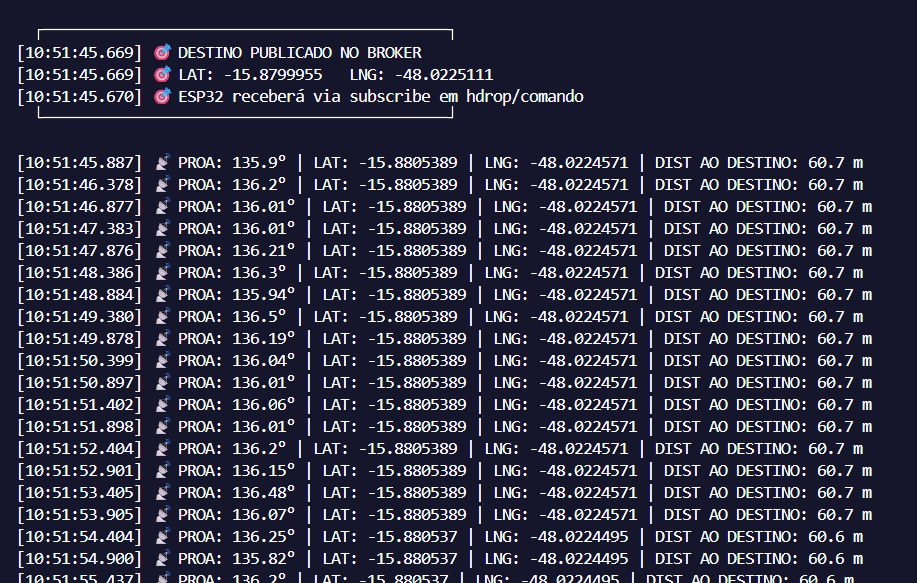
\includegraphics[width=0.6\textwidth]{log_telemetria.jpeg}
\caption{Log de execução: publicação de \textit{waypoints}, cálculo de proa e distância ao destino via MQTT.}
\label{fig:evidencia_firmware}
\end{figure}

No PC4, o módulo A7670SA foi validado em campo: o terminal de geolocalização obteve \textit{fix} GNSS estável e estabeleceu o enlace 4G LTE, transmitindo coordenadas reais (latitude, longitude e curso) para a Estação de Controle. A Figura~\ref{fig:terminal_gnss} mostra o terminal GNSS em funcionamento durante os ensaios.

\begin{figure}[H]
\centering
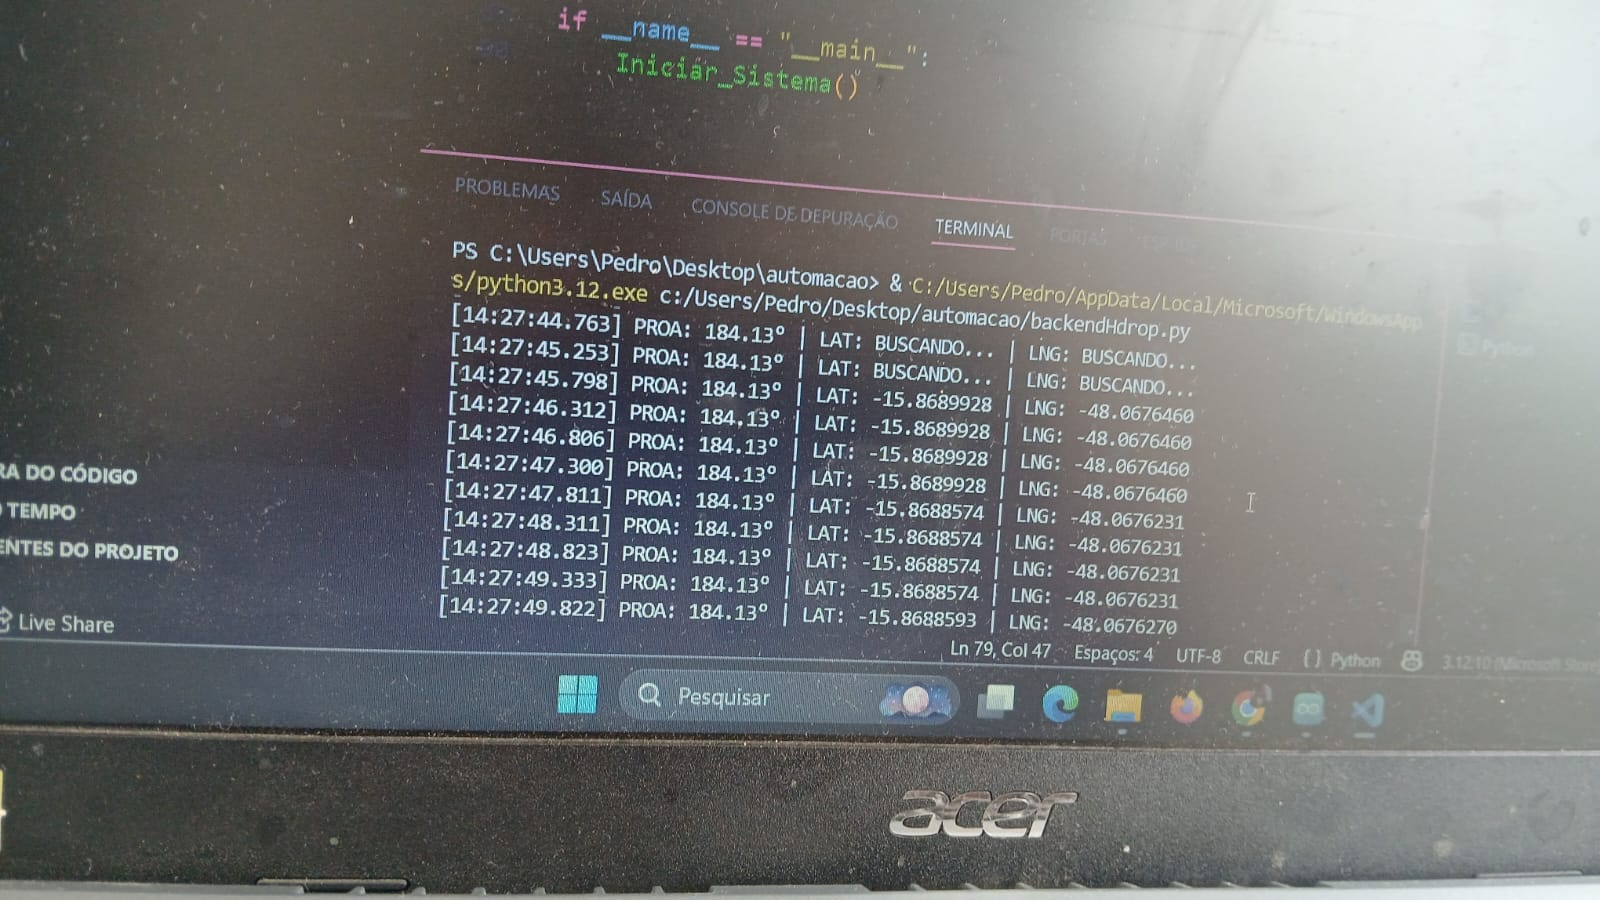
\includegraphics[width=0.6\textwidth]{Terminal_GNSS_funcionando.jpeg}
\caption{Terminal de geolocalização GNSS em funcionamento: aquisição de \textit{fix} e transmissão de coordenadas via 4G.}
\label{fig:terminal_gnss}
\end{figure}

\subsubsection{Estação de Controle de Missão}

A Estação de Controle implementada em Angular~19 recebe o \textit{streaming} de telemetria via WebSocket e renderiza a posição do ASV em mapa Leaflet. O \textit{dashboard} permite o despacho dinâmico de novos destinos por interação direta no mapa. A Figura \ref{fig:evidencia_software} ilustra a interface.

\begin{figure}[H]
\centering
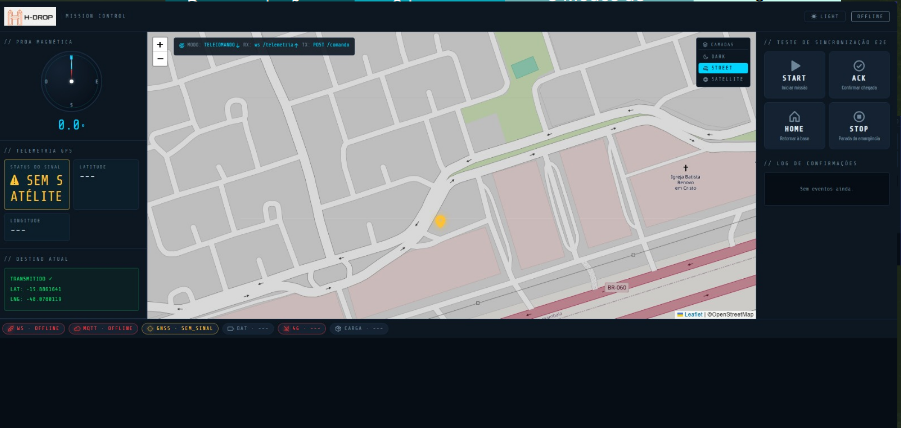
\includegraphics[width=0.8\textwidth]{dashboard_angular.png}
\caption{Estação de Controle de Missão: visualização de telemetria em tempo real e mapa tático.}
\label{fig:evidencia_software}
\end{figure}

\subsubsection{Montagem da Torre de Comunicação e Sensoriamento}
Como elemento de integração entre o hardware de radiofrequência, o \textit{firmware} e a estrutura física, foi construída e acoplada à embarcação uma \textbf{Torre Vertical} em PVC rígido. No PC4 a torre saiu da fase de projeto e foi efetivamente montada na proa do catamarã (Figura~\ref{fig:torre_montada}), elevando as antenas GNSS/4G e o magnetômetro acima do convés. A solução atende, na prática, aos três requisitos técnicos de integração previstos:

\begin{enumerate}
    \item \textbf{Isolamento Eletromagnético da Bússola:} O magnetômetro QMC5883L (I2C nos pinos GPIO21/SDA e GPIO22/SCL) é mantido afastado dos campos magnéticos parasitas gerados pelos motores \textit{brushless} e pelo cabeamento de 12V. A torre eleva o sensor verticalmente, mitigando o efeito \textit{hard-iron} e preservando a precisão do cálculo de proa ($\theta = \operatorname{atan2}(Y,X)$).
    \item \textbf{Desimpedimento do Plano de Terra RF:} A antena ativa de GNSS e a antena de chicote 4G LTE foram posicionadas no topo da torre, desimpedidas da lâmina d'água e de superfícies reflexivas, otimizando o \textit{Time-to-First-Fix} (TTFF) e mantendo estabilidade de rastreamento de satélites.
    \item \textbf{Passagem de Cabeamento e Estanqueidade:} O interior cilíndrico da torre serve como duto para a fiação blindada de sinal e alimentação, direcionada para a caixa estanque inferior por meio de prensa-cabos, eliminando falhas por mau contato mecânico sob vibração.
\end{enumerate}

\begin{figure}[H]
\centering
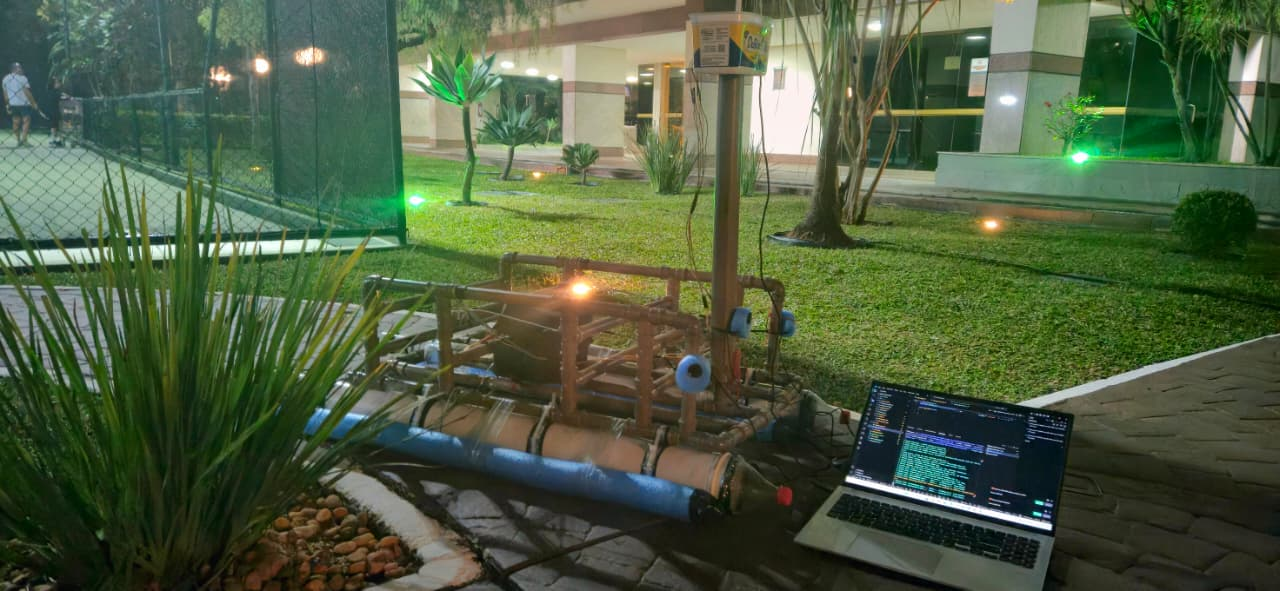
\includegraphics[width=0.5\textwidth]{Projeto Fisico com a Torre.jpeg}
\caption{Protótipo físico do H-DROP com a torre de comunicação e sensoriamento montada na proa.}
\label{fig:torre_montada}
\end{figure}

\subsection{Subsistema de Percepção (Sensoriamento)}

\subsubsection{Validação do Sensor Ultrassônico e Expansão para \textit{Array} de Cobertura Lateral}

Os testes do sensor ultrassônico JSN-SR04T confirmaram a limitação do lóbulo de irradiação de aproximadamente 20°, insuficiente para cobertura lateral da proa em ambiente fluido. A migração para um \textit{array} de três sensores posicionados em leque foi implementada no \textit{firmware}. O filtro de média móvel de 5 pontos reduziu as leituras erráticas causadas por reflexões especulares na água. A Figura \ref{fig:evidencia_sensores} ilustra a bancada de teste.

\begin{figure}[H]
\centering
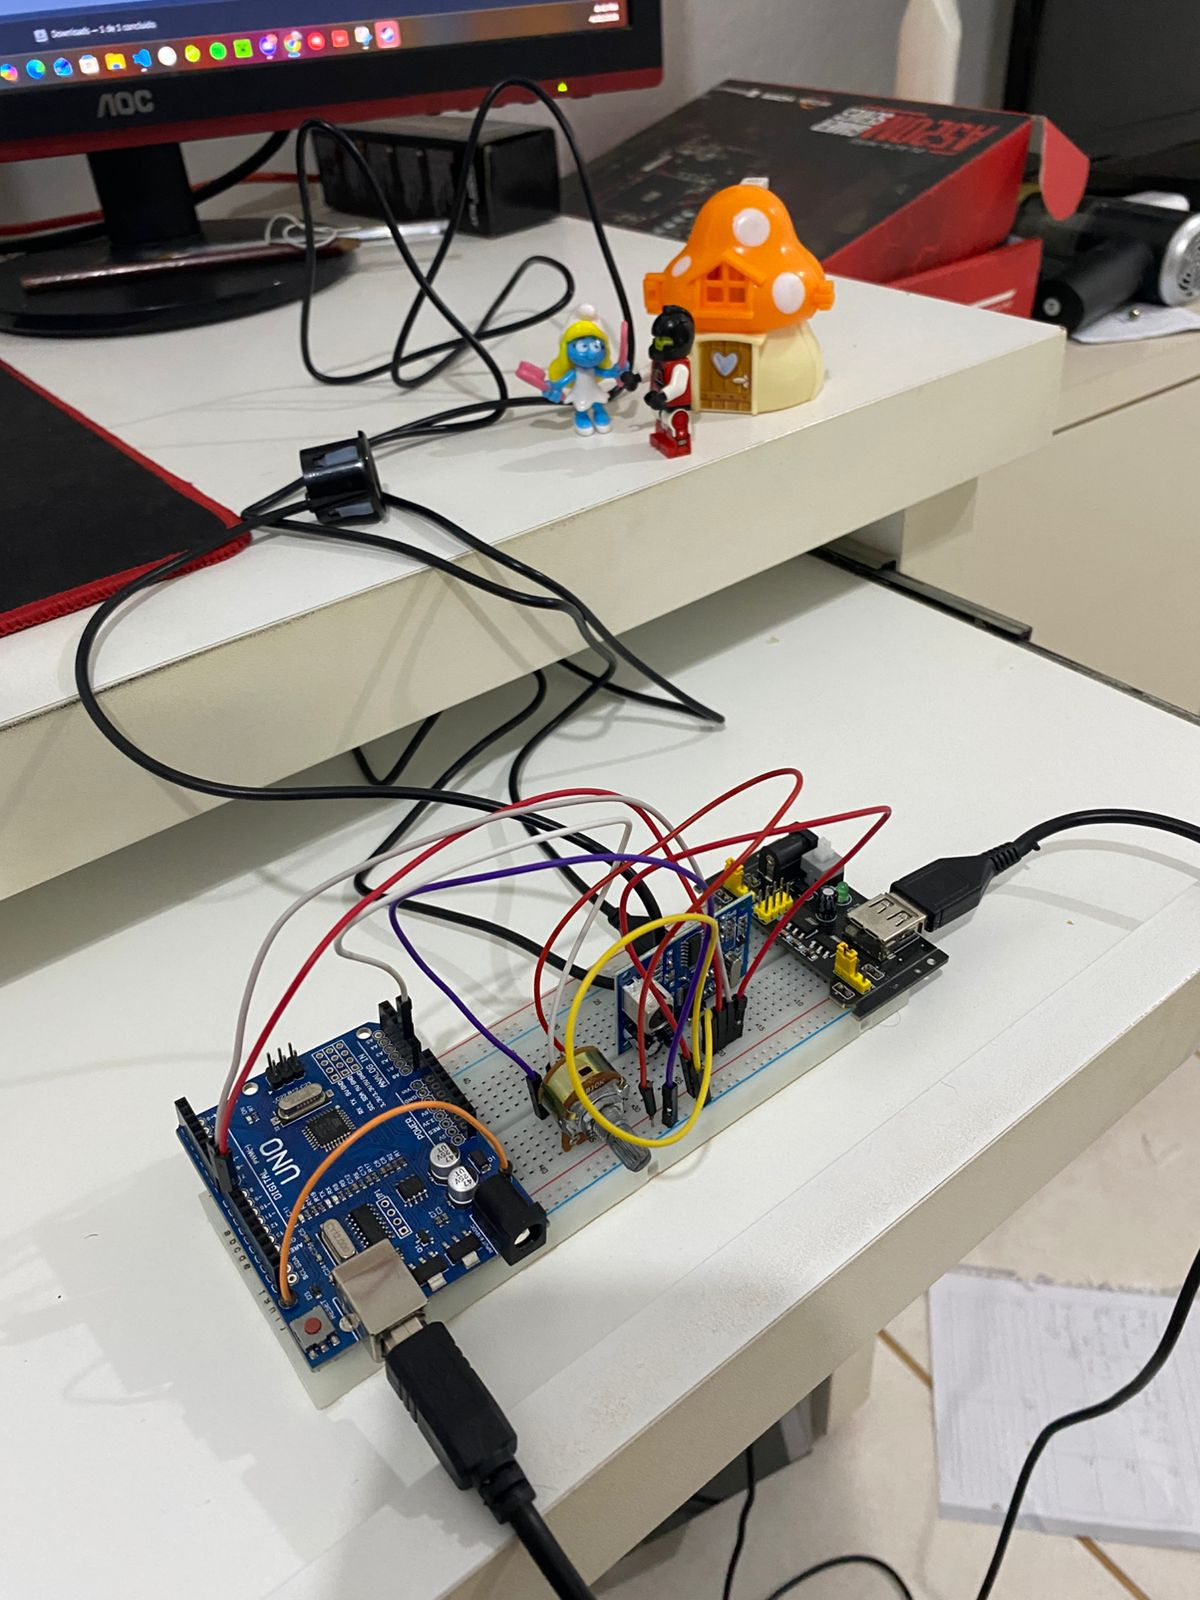
\includegraphics[width=0.4\textwidth]{teste_sensor_ultrassonico.jpeg}
\caption{Bancada de teste do sensor ultrassônico e diagrama de cobertura do lóbulo.}
\label{fig:evidencia_sensores}
\end{figure}

\subsubsection{Validação do Módulo HX711 e LED}
Adicionalmente, foram realizados testes funcionais do módulo HX711 integrado à célula de carga, validando a leitura de peso com resolução de 24 bits via Arduino Nano. A Figura \ref{fig:sensores_laterais} e a Figura \ref{fig:hx711_teste} registram o estado atual da montagem.

\begin{figure}[H]
    \centering
    \begin{minipage}[t]{0.32\textwidth}
        \centering
        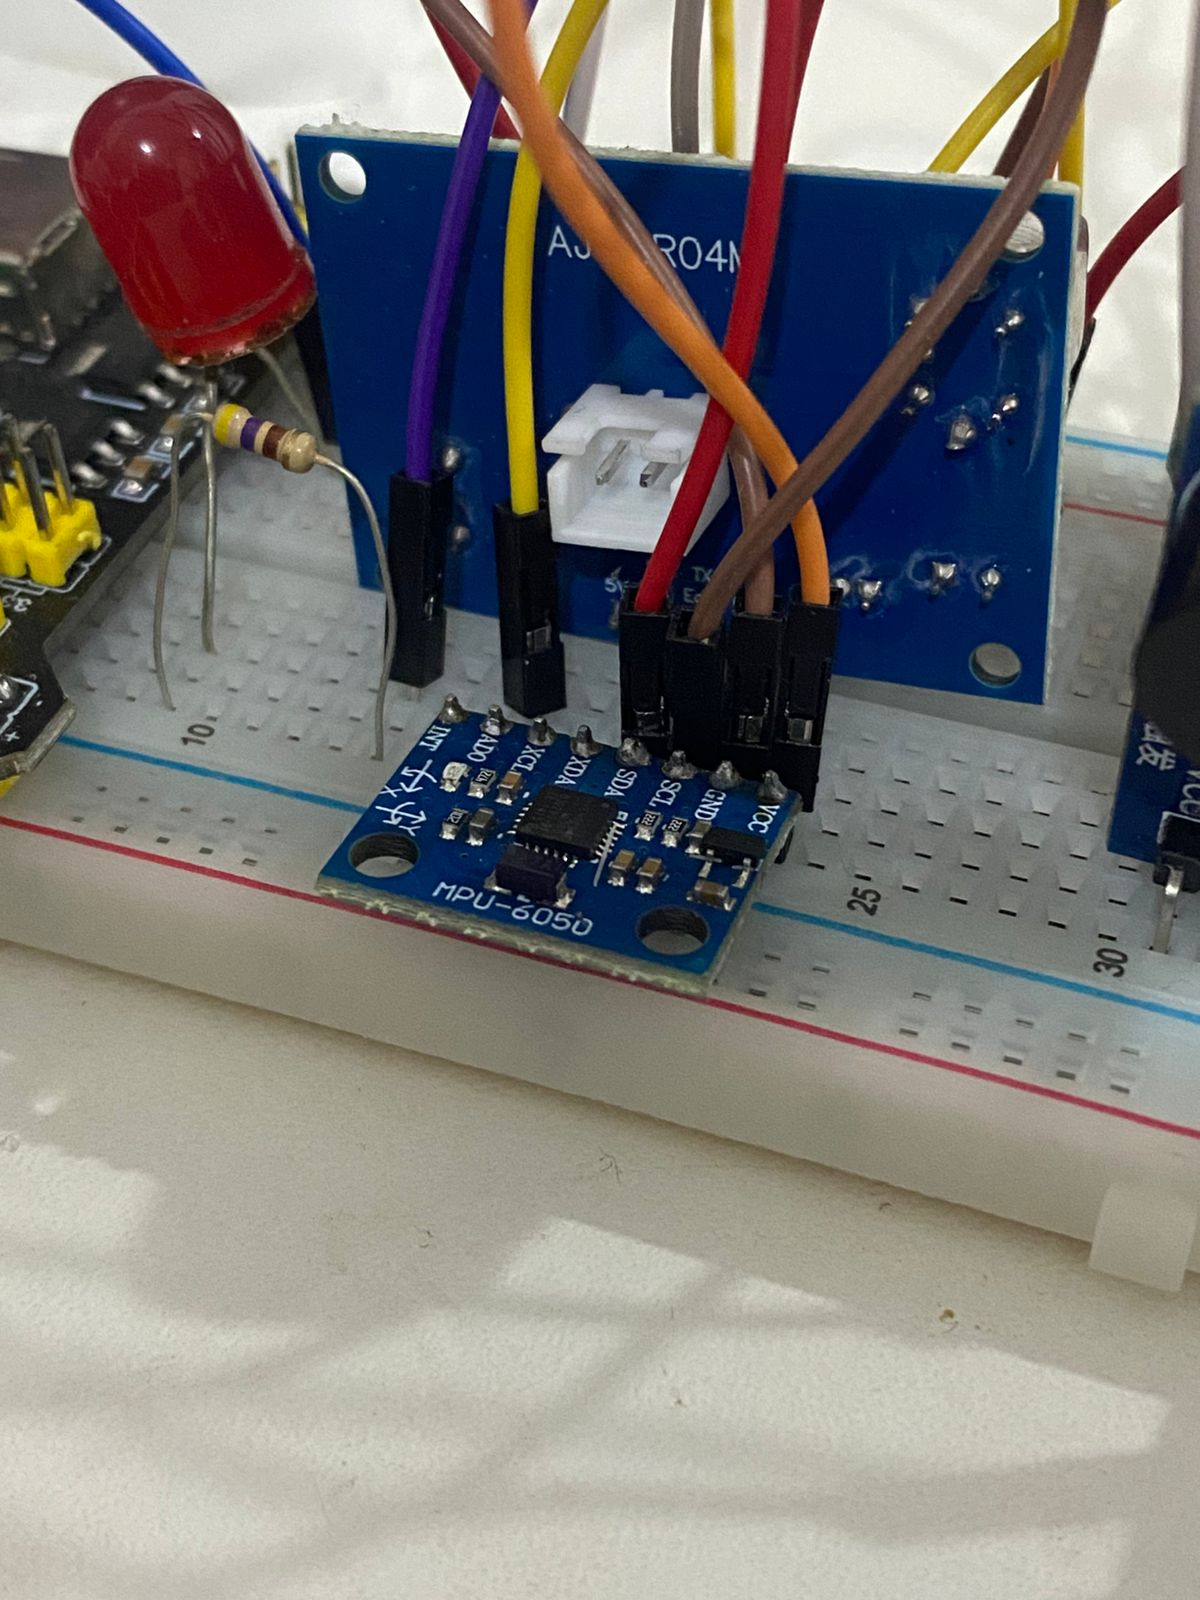
\includegraphics[width=\textwidth]{mpu.jpeg}
        \caption{Montagem do modulo MPU}
        \label{fig:sensores_laterais}
    \end{minipage}
    \hfill
    \begin{minipage}[t]{0.32\textwidth}
        \centering
        \includegraphics[width=\textwidth]{carga.jpeg}
        \caption{Bancada de teste do amplificador HX711 integrado à célula de carga: validação da leitura de peso via Arduino Nano.}
        \label{fig:hx711_teste}
    \end{minipage}
    \hfill
    \begin{minipage}[t]{0.32\textwidth}
        \centering
        \includegraphics[width=\textwidth]{led.jpeg}
        \caption{Led atualmente não montada}
        \label{fig:led_mosfet}
    \end{minipage}
\end{figure}

\subsubsection{Ajuste de Escopo}

O subsistema de sensores não sofreu remoção nem substituição de componentes em relação ao PC2. A evolução registrada neste ponto de controle corresponde a uma \textbf{expansão deliberada} da camada de percepção, motivada pela necessidade de aumentar a cobertura perimetral da embarcação e viabilizar a pesagem da carga útil embarcada.

Três frentes de expansão foram implementadas:

\begin{itemize} 
    \item \textbf{Detecção lateral de obstáculos:} Adição de dois sensores ultrassônicos JSN-SR04T nas laterais do casco (bordo e bombordo), complementando o sensor frontal já existente. O sistema passou a operar com três pontos de cobertura angular simultâneos, ampliando a capacidade de evasão dinâmica em manobras e trechos confinados.

    \item \textbf{Amplificação do sinal da célula de carga:} Integração do módulo amplificador HX711 ao circuito de pesagem. O sinal analógico bruto gerado pela célula de carga possui amplitude insuficiente para leitura direta pelo microcontrolador; o HX711 realiza a amplificação e conversão analógico-digital com resolução de 24 bits, comunicando-se com o Arduino Nano via interface de dois fios (\texttt{DT}/\texttt{SCK}).

    \item \textbf{Sinalização visual por fita LED:} Adição de uma fita de LED 12V para indicação do estado operacional da embarcação. Por operar em 12V e demandar corrente incompatível com a saída direta dos pinos do microcontrolador, o acionamento é realizado por transistor MOSFET IRFZ44N controlado por sinal PWM. O conector P2 fêmea original da fita foi removido para adequação ao circuito de acionamento.
\end{itemize}


\subsection{Integração Física Final da Plataforma}

Na etapa final, todos os subsistemas foram reunidos em uma única plataforma operacional. A torre de comunicação e sensoriamento foi montada na proa (Figura~\ref{fig:torre_montada}), elevando as antenas GNSS/4G e o magnetômetro acima da lâmina d'água e do cabeamento de potência. O barramento de alimentação LiFePO4 foi integrado de forma definitiva a \textbf{todos os módulos de processamento} — a ESP32 (controle, navegação e telemetria) e o Arduino Nano (sensoriamento anticolisão, pesagem e sinalização) — alimentados pelos ramais lógico (\textit{Buck} 5~V) e de tração (ESCs) descritos na Seção de Hardware. Os dois motores BLDC foram \textbf{sincronizados} via ESCs bidirecionais, respondendo de forma coordenada aos comandos diferenciais de avanço, ré e giro sobre o próprio eixo.

A embarcação completa, com a torre instalada e a eletrônica embarcada, foi submetida a \textbf{ensaio em ambiente aquático}, confirmando a flutuabilidade, a estabilidade transversal do catamarã e a integridade do compartimento eletrônico sob a carga real dos subsistemas integrados.

\subsection{Resultados e Discussão}

Esta seção avalia criticamente o desempenho da solução frente aos requisitos estabelecidos ao longo do projeto.

\paragraph{O sistema funcionou como esperado?} Em linhas gerais, sim. A integração estrutural, eletromecânica e de comunicação foi concluída e a plataforma operou de forma coordenada em água. Os subsistemas de estrutura física, propulsão, alimentação, geolocalização e comunicação responderam conforme o projeto. As ressalvas concentram-se na navegação autônoma totalmente não supervisionada, cuja malha de controle ainda depende de sintonização fina em campo.

\paragraph{Quais requisitos foram atendidos?} A Tabela~\ref{tab:atendimento} sintetiza o grau de atendimento por subsistema. Foram plenamente atendidos: a flutuabilidade e a estanqueidade da estrutura (validadas em água com a eletrônica embarcada); a sincronização e o acionamento dos motores pela bateria do projeto; a integração e a proteção do barramento de energia (BMS, \textit{shunt} externo INA226, conector \textit{anti-spark}, diodos Schottky); a aquisição de \textit{fix} GNSS e o enlace 4G LTE validados em campo (Figura~\ref{fig:terminal_gnss}); e a telemetria MQTT com a Estação de Controle em Angular, dentro dos limites de latência e persistência definidos.

\paragraph{Quais requisitos não foram plenamente atendidos?} A navegação autônoma ponto a ponto em malha fechada na água foi exercitada em simulação de alta fidelidade, mas os ganhos do controlador ($K_p$, $K_i$, $K_d$) não foram calibrados em regime real com o conjunto completo de distúrbios hidrodinâmicos. A validação do sistema anticolisão em movimento permaneceu parcial. A reserva de flutuabilidade, sem os flutuadores de EVA, ficou abaixo da meta de projeto de 40\%.

\paragraph{Quais foram as causas prováveis das limitações?} A principal causa é a dependência da disponibilidade simultânea de todo o hardware integrado e de janelas de ensaio em água para o ajuste iterativo do PID — atividade naturalmente posterior à integração física, concluída ao fim do cronograma. Soma-se a ausência de um \textit{driver} de IMU real durante boa parte do desenvolvimento, que manteve o termo derivativo de \textit{heading} ($g_z$) em regime simulado.

\paragraph{O que pode ser melhorado em uma próxima versão?} (i) Calibração sistemática dos ganhos de controle por ensaios instrumentados em água, com registro de telemetria; (ii) instalação dos flutuadores de EVA para elevar a reserva de flutuabilidade acima de 40\%; (iii) fusão inercial com o MPU-6050 real para amortecer a oscilação angular; (iv) integração direta \textit{firmware}↔\textit{broker} MQTT em campo, substituindo o servidor de simulação; e (v) compensação ativa da zona morta dos ESCs no controlador para eliminar o acúmulo indevido do termo integral.

\paragraph{Correções consolidadas.} A queima do ESP32 (PC2) foi corrigida com isolamento termorretrátil e revisão do barramento I2C, sem recorrência. A dessincronização \textit{firmware}/\textit{backend} foi resolvida com padronização da API em \texttt{/api/v1/} e testes de \textit{loopback} via HiveMQ. A instabilidade do 4G por picos de corrente de até 2{,}8~A foi mitigada por capacitores de tântalo, com publicação estabilizada a 2~Hz.

\begin{table}[H]
\centering
\caption{Grau de atendimento dos requisitos por subsistema no PC4}
\label{tab:atendimento}
\renewcommand{\arraystretch}{1.3}
\small
\begin{tabularx}{\textwidth}{|p{3.2cm}|X|c|}
\hline
\rowcolor{gray!20}
\textbf{Subsistema} & \textbf{Requisito-chave} & \textbf{Status} \\ \hline
Estrutura Física (EF) & Flutuabilidade, estabilidade e estanqueidade com eletrônica embarcada (ensaio aquático) & Atendido \\ \hline
\rowcolor{gray!10}
Propulsão (PR) & Sincronização dos motores BLDC e acionamento pela bateria do projeto & Atendido \\ \hline
Gerenc. Energético (GE) & Barramento LiFePO4 + BMS, INA226 com \textit{shunt} externo, proteções elétricas & Atendido \\ \hline
\rowcolor{gray!10}
Geolocalização (GR) & \textit{Fix} GNSS estável e enlace 4G LTE validados em campo & Atendido \\ \hline
Comunicação (CM) & Telemetria MQTT e Estação de Controle (latência/persistência) & Atendido \\ \hline
\rowcolor{gray!10}
Controle (CT) & Navegação autônoma em malha fechada na água com PID calibrado & Parcial \\ \hline
Sensores/Percepção (SP) & Anticolisão em movimento; pesagem e sinalização integradas (ESP32 + Arduino) & Parcial \\ \hline
Estrutura Física (EF) & Reserva de flutuabilidade $\ge 40\%$ (sem flutuadores de EVA) & Não atendido \\ \hline
\end{tabularx}
\end{table}


% ============================================================
\section{Dificuldades Encontradas e Plano de Correção}

A Tabela \ref{tab:dificuldades} apresenta os principais desafios enfrentados ao longo do desenvolvimento até o PC3.

\footnotesize
\begin{longtable}{| p{0.28\textwidth} | p{0.30\textwidth} | p{0.32\textwidth} |}
\caption{Dificuldades encontradas e plano de correção} \label{tab:dificuldades} \\
\hline
\textbf{Dificuldade / Desafio} & \textbf{Causa e Impacto} & \textbf{Ação Corretiva} \\ \hline
\endfirsthead
\hline
\textbf{Dificuldade / Desafio} & \textbf{Causa e Impacto} & \textbf{Ação Corretiva} \\ \hline
\endhead

\textbf{Queima do ESP32} & \textbf{Causa:} Terminal do magnetômetro QMC5883L solto encostou na linha de 12~V do Buck. \newline \textbf{Impacto:} Perda imediata do microcontrolador por sobretensão. & Substituição imediata; revisão do barramento I2C; isolamento termorretrátil em todos os terminais expostos. \\ \hline

\textbf{Lóbulo insuficiente do ultrassônico} & \textbf{Causa:} Ângulo de irradiação do JSN-SR04T ($\approx 20°$) insuficiente para cobertura lateral da proa. \newline \textbf{Impacto:} Pontos cegos na navegação autônoma. & Migração para \textit{array} de três sensores em leque. Filtro de média móvel de 5 pontos no \textit{firmware}. \\ \hline

\textbf{Divergência CAD vs. manufatura} & \textbf{Causa:} Indisponibilidade de conexões de PVC com ângulos específicos no mercado local. \newline \textbf{Impacto:} Tensões mecânicas não previstas no chassi. & Redesign pontual com assentamento por pressão (macetes). Flutuadores auxiliares de EVA previstos para compensar microfissuras. \\ \hline

\textbf{Instabilidade do 4G LTE} & \textbf{Causa:} \textit{Bursts} de até 2{,}8~A durante transmissões MQTT causavam quedas no barramento lógico. \newline \textbf{Impacto:} Reinicializações do módulo A7670SA. & Capacitores de tântalo de 1000~$\mu$F em paralelo à alimentação. Publicação ajustada para 2~Hz. \\ \hline

\textbf{Dessincronização Firmware vs. Backend} & \textbf{Causa:} Diferença na abstração dos esquemas JSON entre C++ e Angular. \newline \textbf{Impacto:} Erros de \textit{parsing} na Estação de Controle. & Padronização da API em \texttt{/api/v1/}. Testes de \textit{loopback} via HiveMQ. \\ \hline

\end{longtable}
\normalsize

% ============================================================
\section{Planejamento de Montagem, Testes e Validação}

\subsection{Planejamento de Montagem}

O desenvolvimento foi dividido em três frentes simultâneas, mantidas e consolidadas desde o PC2:

\begin{itemize}
\item \textbf{\textit{Software-in-the-Loop}:} Injeção de dados simulados (GNSS, magnetômetro, ultrassônico) diretamente no ESP32 via Estação de Controle e \textit{broker} MQTT, validando a lógica PID e os filtros.
\item \textbf{Integração Eletromecânica em Bancada:} União da bateria LiFePO4, BMS, INA226, ESCs e motores fora d'água, calibrando o algoritmo de Contagem de Coulomb e o \textit{throttling} por nível de carga.
\item \textbf{Montagem Estrutural:} Finalização do chassi em PVC, instalação da torre de sensores e integração completa da eletrônica ao casco.
\end{itemize}

\subsection{Validação Inicial (Prova de Conceito)}

A Prova de Conceito será validada com sucesso ao cumprir os seguintes critérios:

\begin{enumerate}
\item A embarcação demonstra navegação autônoma estável, orientada pela fusão de dados GNSS e bússola inercial.
\item O subsistema de controle realiza evasão dinâmica ao detectar obstáculos via sensores ultrassônicos.
\item A Estação de Controle recebe e processa pacotes de telemetria (posição, energia e latência 4G) sem interrupções críticas.
\item Os compartimentos internos apresentam ausência total de umidade após a missão.
\end{enumerate}

% ============================================================
\section{Conclusão}

O H-DROP percorreu, ao longo do semestre, a trajetória completa do modelo puramente conceitual (PC1) ao protótipo físico integrado e validado (PC4). Neste estágio final, todos os subsistemas foram reunidos em uma única plataforma funcional: a estrutura em PVC com a torre de comunicação montada, a propulsão diferencial com motores sincronizados, o barramento de alimentação LiFePO4 com BMS acoplado a todos os módulos de processamento (ESP32 e Arduino), o subsistema de geolocalização e comunicação 4G/GNSS validado em campo e o \textit{firmware} de controle e telemetria sobre FreeRTOS. A embarcação completa foi ensaiada em ambiente aquático.

\textbf{Principais resultados e grau de atendimento dos objetivos:} foram plenamente atingidos os objetivos de plataforma flutuante estável, propulsão sincronizada, gerenciamento de energia protegido, geolocalização/comunicação móvel e telemetria com Estação de Controle. O objetivo de navegação autônoma ponto a ponto foi alcançado em ambiente de simulação de alta fidelidade e validado parcialmente em água, restando a calibração fina da malha de controle.

\textbf{Limitações finais:} a sintonização dos ganhos do controlador em malha fechada na água e a validação plena do anticolisão em movimento permanecem como frentes de refinamento; a reserva de flutuabilidade, sem os flutuadores de EVA, ainda está abaixo da meta de 40\%.

\textbf{Aprendizados técnicos:} a integração de cargas de alta corrente (motores/4G) com eletrônica sensível exigiu defesa em profundidade — separação de ramais, \textit{anti-spark}, diodos Schottky, \textit{shunt} externo e capacitores de amortecimento. A migração para um \textit{array} de sensores e a adoção de \textit{firmware} assíncrono sobre FreeRTOS mostraram-se decisivas para a robustez do sistema. O ambiente de simulação em três camadas permitiu amadurecer o algoritmo de navegação antes do contato com a água, reduzindo risco.

\textbf{Trabalhos futuros:} calibração instrumentada do PID em água; instalação dos flutuadores de EVA; fusão inercial com MPU-6050 real; integração direta \textit{firmware}↔MQTT em campo; e compensação ativa da zona morta dos ESCs.

\textbf{Avaliação crítica do processo:} o desenvolvimento incremental por pontos de controle, com validação independente de cada subsistema antes da integração total, mostrou-se eficaz para conter falhas sistêmicas. O principal gargalo foi a dependência da integração física completa para liberar os ensaios de controle em malha fechada, concentrados ao fim do cronograma — um aprendizado a antecipar em projetos futuros.

% ============================================================
\section{Cronograma de Desenvolvimento e Entregas}

\begin{table}[h!]
\centering
\caption{Cronograma Detalhado de Atividades — Maio e Junho de 2026}
\label{tab:cronograma_detalhado}
\renewcommand{\arraystretch}{1.3}
\begin{tabular}{|c|p{0.33\textwidth}|p{0.45\textwidth}|}
\hline
\rowcolor{gray!20}
\textbf{Data} & \textbf{Equipes Envolvidas} & \textbf{Atividade / Marco de Entrega} \\ \hline
02/05 & Controle e Geolocalização & Desenvolvimento e testes de bancada do subsistema de controle e fusão de dados. \\ \hline
07/05 & Alimentação e Propulsão & Montagem final do barramento de potência e testes de empuxo dos motores. \\ \hline
12/05 & Sensores de Colisão & Implementação do novo sensor de redundância para melhoria da zona cega. \\ \hline
18/05 & Website e Controle & Finalização do software, integração via MQTT e testes de telemetria em tempo real. \\ \hline
23/05 & Geral (Integração) & Montagem completa do hardware no casco e vedação estanque. \\ \hline
\textbf{28/05} & \textbf{Todas as Equipes} & \textbf{Entrega do PC3: Integração Completa Hardware/Software.} \\ \hline
04/06 & Geolocalização e Controle & Coleta de dados em ambiente aquático e calibração do PID (Giro Zero). \\ \hline
11/06 & Sensores e Website & Validação do sistema anticolisão em movimento; logs de telemetria via 4G. \\ \hline
18/06 & Geral (Validação) & Ensaios de curso para autonomia e estabilidade estrutural. \\ \hline
23/06 & Documentação & Consolidação de resultados, gráficos de consumo energético e logs. \\ \hline
\textbf{25/06} & \textbf{Todas as Equipes} & \textbf{Entrega Final do PC4: Relatório de Desempenho e Validação.} \\ \hline
\end{tabular}
\end{table}

% ============================================================
\printbibliography[title={Referências}]
\nocite{*}

% ============================================================
\section{Anexos}

Os materiais complementares a seguir foram referenciados ao longo do relatório e são reunidos aqui para preservar a fluidez da leitura.

\begin{itemize}
\item \textbf{Imagens da montagem física:} comparativo CAD vs.\ construído (Figura~\ref{fig:evidencia_estrutura}), torre de comunicação montada (Figura~\ref{fig:torre_montada}), ensaio de flutuabilidade (Figura~\ref{fig:flutuabilidade}) e prototipagem eletrônica (Figura~\ref{fig:evidencia_eletronica}).
\item \textbf{Capturas de esquemáticos e diagramas:} esquemático de navegação/telemetria (Figura~\ref{fig:esquematico_pc3}), diagrama de blocos da arquitetura (Figura~\ref{fig:diagrama_controle_detalhado}), arquitetura de controle cíclica (Figura~\ref{fig:arquitetura_controle_ciclica}), diagrama de alimentação (Figura~\ref{fig:diagrama_alimentacao}) e topologia do barramento de potência (Figuras~\ref{fig:topologia1} e~\ref{fig:topologia2}).
\item \textbf{Capturas de comunicação e telemetria:} log de telemetria MQTT (Figura~\ref{fig:evidencia_firmware}), terminal GNSS em funcionamento (Figura~\ref{fig:terminal_gnss}) e Estação de Controle em Angular (Figura~\ref{fig:evidencia_software}).
\item \textbf{Prints de simulação:} \textit{dashboard} de controle (Figura~\ref{fig:dashboard_geral}), mapa tático da rota A→B e log de eventos da FSM.
\item \textbf{Registros de testes de sensores:} bancada do ultrassônico (Figura~\ref{fig:evidencia_sensores}) e módulos MPU/HX711/LED (Figuras~\ref{fig:sensores_laterais}--\ref{fig:led_mosfet}).
\item \textbf{Tabelas de medições e parâmetros:} matriz de componentes (Tabela~\ref{tab:componentes_riscos}), requisitos técnicos (Tabela~\ref{tab:requisitos_tecnicos}), envelope de potência dos ESCs (Tabela~\ref{tab:envelope_pwm}) e grau de atendimento (Tabela~\ref{tab:atendimento}).
\item \textbf{Vídeos de validação:} acionamento dos motores em bancada — \url{https://photos.app.goo.gl/3MceCbJM5Kov54rX7}.
\item \textbf{Trechos de código e repositórios:} código-fonte completo do projeto em \url{https://github.com/AlphaCompLabs/H-Drop.git} — \textit{firmware} de motores em \texttt{/Motors-Simulation} e ambiente de simulação de controle em \texttt{/Controler-Simulation}.
\end{itemize}

% ============================================================
% FIM DO DOCUMENTO
% ============================================================

\end{document}